\chapter{Junk Radiation in Binary Black Hole Simulations}

\section{Chapter Overview}

An Overview of my chapter here.


\section{Chapter TDL}
\begin{itemize}

\item Many citations in the introduction and very much out of
  date. It should be re-written.

\item Are there any new papers on junk radiation to discuss that have
  come out since this time? Ask Harald / do a literature search.

\item Discuss more about boundary conditions in IVP for bbh

\item Maybe make a table detailing all the simulations that were
  done. Come up with a better naming system for the runs.

\item There is a note about the uncertainity from numerical
  trunctation in $E_J$ for SKS. Not sure what to do about that. I
  think it can reasonably left the way it is.

\item Combine data into a single plot for wave extraction plot

\item Decide what to do for $\delta M$ for SKS, given that the data is
  so weird

\item Write the results section closely citing all the figures
  properly. Are we overfitting the data? Be careful with how to report
  the data. Maybe just focus on the plots, and not the fits.

\item Write a conclusion. What are the implications of these kinds of
  numbers?

\end{itemize}


\section{Introduction}
The inspiral and merger of solar-mass binary black holes are one of
the most promising sources for ground-based gravitational wave
detectors such as LIGO~\cite{Barish:1999},
Virgo\cite{Acernese-etal:2006}, and LCGT\cite{Kuroda:2010}. In the
next few years, as it is upgraded to higher sensitivity, Advanced
LIGO is expected to begin making detections, with a realistic event
rate estimated at about 20 per year \cite{Abadie:2010cfa}.
For the gravitational radiation to be detected, and to learn about the
properties of the source, waveform templates must be accurately
modelled.  Although analytic prescriptions like Post-Newtonian (PN)\cite{Blanchet2006} or
Effective One-Body (EOB)\cite{Buonanno99} can accurately model some of the inspiral,
Numerical Relativity (NR) simulations are needed to accurately model
late inspiral and merger of the black holes.

In current NR simulations, there is always a burst of spurious
gravitational radiation at the start of the simulation, often referred to as
``junk radiation''. This pulse
always occurs at the start of the simulation, it is of much higher frequency and amplitude
than the astrophysical gravitational radiation, and it has significant
contributions from modes other than the standard $(l,m) = (2,2)$
spherical harmonic mode, which is the dominant contribution for the
astrophysical part of the waveform.  Therefore, this pulse is not astrophysical.

We illustrate this effect in Fig.~\ref{fig:Typical}, showing the
gravitational waveform  at the start of a
typical simulation. The waves are extracted on a coordinate sphere at
$r=160M$ \footnote{We use units where $G=c=1$. The only natural length
  and time scale is then the total mass of both black holes, $M$.}, so
the waves start appearing at $t\approx 160M$. We see the burst of junk
radiation last about $100M$ in time, with significant contributions
from both the $(2,2)$ and $(2,0)$ modes. The junk radiation then dies out,
and subsequently, the expected sinusoidal $(2,2)$ mode emerges.

\begin{figure}
 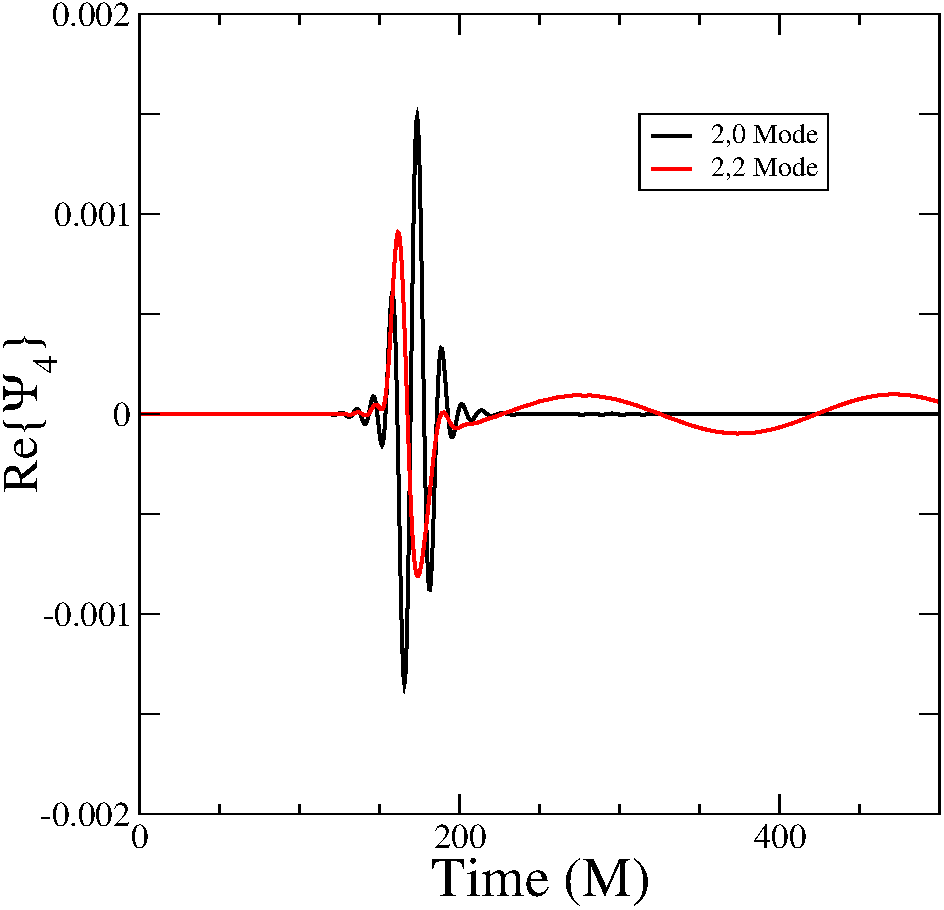
\includegraphics[scale=0.95]{chap5/Typical}
  \caption[A typical run illustrating junk radation.]{A typical run illustrating the spurious burst of junk radiation. We see at early times a burst of high-frequency, high-amplitude radiation. At later times, the $(2,0)$ mode dies out, and the $(2,2)$ mode settles into the usual inspiral-type radiation}
  \label{fig:Typical}
\end{figure}


This junk radiation is undesirable in simulations for several
reasons. It adds to the computational cost of the simulation as the
junk radiation must leave the computational grid before any useful
physical information can be extracted.  It can unrealistically shorten
the time until the black holes
merge\cite{BodeEtAl:2008}. It also makes it more difficult
to compare general relativistic simulations with Post-Newtonian
calculations. It is therefore a useful endeavour to try to better
understand the junk radiation, how important it is, and how to reduce
it.

Junk radiation is thought to be caused by assumptions made during the
initial data construction, which are not compatible with black holes in perfect equilibrium. Specifically,
 black holes are generally treated in the
initial data as independent and non-interacting, while in reality
there should be some non-trivial tidal interactions between them. If
we imagine a sequence of initial data sets where the initial
separation between the holes is decreasing, we would expect that this
effect becomes more important as the initial separation decreases. 
Moreover, the black holes in the initial data are often constructed
with techniques that do not even allow to construct a single, equilibrium black  hole.  Specifically, often, conformal flatness is assumed. As detailed in section~\ref{subsec:IVP}, the construction of initial data has a
free choice for the conformal metric, $\tilde{g}_{ij}$, on the initial
hypersurface. A common choice is conformal flatness, i.e.,
$\tilde{g}_{ij}$ is equal to the flat Euclidean metric. Since every
spherically symmetric space is conformally flat, this would be fine
for one Schwarzchild black hole. However,  a
binary system of compact objects is not conformally flat at second PN
order\cite{Rieth:1997}, and the Kerr space-time does not admit a
conformally flat slicing~\cite{GaratPrice:2000} that continuously approach Schwarzschild coordinates as the spin goes to zero. 
The former effect should decrease in importance with increasing separation of the binary.  The latter is caused by a deficiency of conformally flat slicing that is present even for single spinning black holes, and so we expect its importance
to be approximately independent of binary separation.
% It is reasonable to think that the latter
% effect becomes more important for initial data where the black holes
% have higher spins, while we might imagine that the first effect is
% some sort of constant effect.

Lovelace~\cite{Lovelace2009} investigated the effects on junk radiation of using
superposed Kerr-Schild~\cite{Matzner1999,Marronetti-Matzner:2000,Pfeiffer2002a,Lovelace2008} (conformally curved) initial data for equal mass, non-spinning black
holes.  The metric is written as
\begin{equation}
\tilde{g}_{ij}=f_{ij}+e^{-(r_A/w)^2}\left(g_{ij}^A-f_{ij}\right)+e^{-(r_B/w)^2}\left(g_{ij}^B-f_{ij}\right),
\end{equation}
where $f_{ij}$ is the Euclidean metric, $r^{A,B}$ are the distances
from black holes $A$ and $B$, and $g_{ij}^{A,B}$ is the Kerr-Schild metric boosted in
the direction of the black hole's motion. This has the effect that the
metric looks like Schwarzschild near the black holes, and looks flat
far away. The Gaussian scalings were needed to help improve the
convergence of the initial data. It was found that in general, the
conformally curved initial data can decrease the amplitude of the junk
radiation by a factor of $\sim 2$.
Superposed Kerr-Schild initial data is built around the
  Kerr-Schild metric, which exactly represents single spinning black holes.
 Therefore, one would expect that the advantages of superposed Kerr-Schild become particularly apparent for spinning black holes.

In this paper we investigate the parameter space dependence of junk
radiation. We measure its dependence on the spin and on the initial
separation of the black holes, for low eccentricity, equal-mass,
spin-aligned binaries. We also perform a comparison between conformally
flat initial data, and superposed Kerr-Schild initial data.

The paper is organized as follows: 
  Section~\ref{sec:NumericalMethods} presents the numerical methods,
  and Section~\ref{sec:Methodology} describes how we quantify junk
  radiation and other initial transients in the BBH initial data sets.
  We present our results in Sec.~\ref{sec:Results} and close with a discussion in Sec.~\ref{sec:Discussion}.

\section{Numerical Methods}
\label{sec:NumericalMethods}

\subsection{The Initial Value Problem}
\label{subsec:IVP}
Employing the usual 3+1 decomposition(~\cite{ADM,york79}),space-time is foliated by a family
of spacelike hypersurfaces $\Sigma_t$. Each hypersurface has a
future-pointing unit normal $n^{\mu}$, induced metric $g_{ij}$, and
extrinsic curvature
$K_{\mu\nu}=-\frac{1}{2}\mathcal{L}_{n}g_{\mu\nu}$. The metric is
written as 
\begin{equation}
g_{\mu\nu}=-\alpha^2dt^2+g_{ij}\left(dx^i+\beta^idt\right)\left(dx^j+\beta^jdt\right),
\end{equation}
where $\alpha$ and $\beta$ are the lapse function and the shift vector
respectively. The lapse measures the proper time between neighbouring
hypersurfaces, and the shift vector determines how coordinate labels
move between neighbouring hypersurfaces.  On the initial
hypersurface $\Sigma_0$, spatial metric and extrinsic curvature must satisfy the vacuum
constraint equations
\begin{eqnarray}
R+K^2-K_{ij}K^{ij}&=&0, \\
\nabla_j\left(K^{ij}-g^{ij}K\right)&=&0.
\end{eqnarray}
% They are then evolved in time by the vacuum evolution equations
% \begin{eqnarray}
% \partial_tg_{ij}&=& blahblah \\
% \partial_tK_{ij}&=& blahblah 
% \end{eqnarray}
To solve the constraint equations \ one writes(~\cite{Lichnerowicz44})
the metric in terms of a conformal metric $\tilde{g}_{ij}$ and a
conformal factor $\Psi$:
\begin{equation}
g_{ij}=\Psi^4\tilde{g}_{ij}.
\end{equation}
We also split the extrinsic curvature into trace and trace-free parts
\begin{equation}
K^{ij}=A^{ij}+\frac{1}{3}g^{ij}K,
\end{equation}
and employ the extended conformal thin sandwich formalism~\cite{York1999,Pfeiffer2003b} to further
decompose $A^{ij}$.  One must then choose
$\left(\tilde{g}_{ij},\partial_{t}\tilde{g}_{ij},K,\partial_{t}K\right)$
as the free data.  Compared to the extrinsic curvature decomposition~\cite{Murchadha-York:1974b}, the conformal thin sandwich formalism allows for 
physically motivated choices to a larger number of the free data.  Elliptic equations
with appropriate boundary conditions are then solved for $\Psi$,
$\alpha\Psi$, and $\beta^i$, and the physical data is
re-assembled. $\partial_t\tilde{g}_{ij} = \partial_tK = 0$ is chosen
so that system is initially stationary in the co-rotating
frame.  This then leaves $\tilde{g}_{ij}$ and $K$ as the free data to
choose.  

The two types of initial data we compare are described in detail in
Ref.~\cite{Lovelace2008}: Conformally flat, quasi-equilibrium initial
data employs conformal flatness, maximal slicing ($K=0$) and inner
boundary conditions that enforce that the black holes are
instantaneously in
equilibrium~\cite{Caudill-etal:2006,Cook2004,Cook2002}.  Superposed
Kerr-Schild initial data, first used
in~\cite{Marronetti-Matzner:2000,Matzner1999}, takes the spatial
metric and extrinsic curvature as superposition of elements of
Kerr-Schild metrics (one for each black hole).  As explained in
Ref.\cite{Lovelace2008}, we introduce Gaussian attenuation functions
to ensure regularity at spatial infinity.  Inner boundary conditions
are \red{PROVIDE DETAILS}.



\subsection{Code}
\label{sec:Code}

The initial data is solved using the spectral solver {\tt Spells}(~\cite{Pfeiffer2003}) of the Spectral 
 Einstein Code {\tt SpEC}~\cite{SXSWebsite}.  This is a
multi-domain elliptic PDE solver that uses pseudo-spectral methods,
whereby quantities of interest are expressed as a linear summation of
basis functions. This method gives exponential convergence (with the
number of basis functions) as long as the quantities of interest are
smooth. The black hole singularities are dealt with by excision from
the computational grid. We use the dual frame method described in
\cite{Scheel2006}. The domain decomposition and position of the black
holes are fixed in a comoving frame, but the equations of motion are
solved in an inertial frame that is asymptotically Minkowski. The
frames are related by a rotation term (due to orbital motion) and a
contraction term (due to inspiral motion).

Gravitational waves are extracted on outer spherical shells of the
domain using the Newman-Penrose scalar $\Psi_4$. Given a spacelike
hypersurface with unit normal $n^{\mu}$ and a spatial unit vector in
the direction of wave propagation $r^{\mu}$, $\Psi_4$ is defined as 
\begin{equation}
\Psi_4 = -C_{\alpha\mu\beta\nu}l^{\mu}l^{\nu}m^{\alpha}\bar{m}^{\beta}
\end{equation}
where $C_{\alpha\mu\beta\nu}$ is the Weyl tensor,
$l^{\mu}=\left(n^{\mu}-r^{\mu}\right)/\sqrt{2}$ and $m^{\mu}$ is a
complex null vector satisfying $m^{\mu}\bar{m}_{\mu}=1$. We then expand
$\Psi_4$ in spin-weighted spherical harmonics
\begin{equation}
\Psi_4(t,r,\theta,\phi)=\sum_{l,m}{\Psi_4^{lm}(t,r)_{-2}Y_{lm}(\theta,\phi)}
\end{equation}
The number of terms used in this expansion is generally $l\le 8$ in
our simulations. At large $r$, $\Psi_4$ is related to the
gravitational wave amplitude, $h$, by
\begin{equation}
\Psi_4=\frac{d^2}{dt^2}h_{+}-i\frac{d^2}{dt^2}h_{\times}.
\end{equation}


\subsection{Eccentricity Reduction}
Gravitational radiation tends to circularize in-spiralling compact
binaries(~\cite{PetersMathews1963,Peters1964}). We reduce orbital
eccentricity with an iterative method similar to the one described in~\cite{Boyle2007,Chu2009}. One guesses the initial orbital
frequency $\Omega_0$ from Kepler's third law or from a Post-Newtonian
calculation, while assuming that the initial radial velocity, $v_r$ is
zero. After the first simulation has run for a sufficient length, about two orbits, we fit the time derivative of
the orbital frequency, $\dot{\Omega}(t)$ as suggested
in~\cite{Buonanno:2010yk}.  We fit parameters $\{A_0, A_1, T_c, B, \phi, \omega, q\}$ with the function
\begin{equation}
\dot{\Omega}(t)=A_0\left(T_c-t\right)^{-11/8}+A_1\left(T_c-t\right)^{-13/8}
+B\cos\left(\varphi + \omega
  t+qt^2\right),
\end{equation}
where $T_C$ is the time of merger. The first two terms represent the
smooth inspiral motion of the black holes, while the oscillatory
second terms represents unwanted effects due to eccentricity. The
updating formulae
\begin{equation}
\delta\Omega_0=-\frac{B\omega\sin{\varphi}}{4\Omega_0^2}
\end{equation}
\begin{equation}
\delta v_r = \frac{B d_0\cos{\varphi}}{2\Omega_0},
\end{equation}
where $d_0$ is the binary separation, are designed to circularize low eccentricity Newtonian binaries. This
process is continued iteratively, typically another one or two times,
until the eccentricity is reduced to $e\lesssim 0.002$. The effect of
eccentricity on junk radiation is discussed in section~\ref{subsec:ErrorEstimation}.

%
%\begin{eqnarray}
%\dot{\Omega}(t)&=&A_0\left(T_c-t\right)^{-11/8}+\\
%&&A_1\left(T_c-t\right)^{-13/8}+B\cos\left(\omega
 % t+\varphi+qt^2\right)
%\end{eqnarray}

%Gravitational radiation tends to circularize in-spiralling compact objects~\cite{PetersMathews1963,Peters1964}.  We reduce orbital eccentricity with an 
%iterative method similar
%to the one described in Refs.\cite{Boyle2007,Chu2009}.  One 
%guesses the initial orbital frequency $\Omega_0$ from Kepler's law or
%a Post-Newtonian calculation, while assuming that the initial radial
%velocity is zero. The time derivative of the black holes is then fit
%with five parameters
%\begin{equation}
%\dot{d}(t)=A_0+A_1t+B\sin(\omega t+\varphi)
%\end{equation}
%The first two terms represent the smooth inspiral motion of the holes,%
%while the \{oscillatory} second term represents unwanted effects due to
%eccentricity. In a Newtonian orbit, the eccentricity would be
%\begin{equation}
%e=\frac{B}{\omega d_0}.
%\end{equation}
%The values of $\Omega_0$ and $v_r$ are adjusted to make $B$ as small
%as possible, using
%\begin{equation}
%\delta\Omega_0=-\frac{B\omega\cos{\varphi}}{2d_0\Omega_0},
%\end{equation}
%\begin{equation}
%\delta v_r = -\frac{B\sin{\varphi}}{2}.
%\end{equation}
%These formulae are designed such that they circularize
%low-eccentricity Newtonian orbits. This process is continued
%iteratively, typically once or twice, until the
%eccentricity reduced to  $e\lesssim 0.002$.

%\red{[Only describe what you do: Combine the preceding and following
 % paragraphs, only leaving the equations you do actually use.]}
%In our simulations we used a similar procedure, but instead we fit
%the time-derivative of the orbital frequency, $\dot{\Omega}$, as suggested
%in~\cite{Buonanno:2010yk}. The fit is
%\begin{eqnarray}
%\dot{\Omega}(t)&=&A_0\left(T_c-t\right)^{-11/8}+\\
%&&A_1\left(T_c-t\right)^{-13/8}+B\cos\left(\omega
 % t+\varphi+qt^2\right)
%\end{eqnarray}
%and the updating formulae are:

%\begin{equation}
%\delta\Omega_0 = -\frac{B\omega\sin{\varphi}}{4\Omega_0^2}
%\end{equation}red
%\begin{equation}
%\delta v_r = \frac{B d_0}{2\Omega_0}\cos{\varphi}
%\end{equation}

%The effect of orbital eccentricity on junk radiation is discussed in
%section ~\ref{subsec:EccentricityEffect}

\subsection{Simulations}

We run BBH evolutions using both conformally flat and SKS initial
data.  We consider five different initial separations for CF data,
$D/M=\{12,15,20,25,30\}$, and $D/M=\{12,15,20\}$ for SKS data, where $M$ is the total mass of both black
holes, and at each separation we consider  six different spins,
$\chi=\{0,0.1,0.2,0.3,0.4,0.5\}$. In each case the black holes are of
equal mass, equal spin, and the spin is aligned with the orbital
angular momentum, i.e., in the the $+z$ direction. To test the
convergence of quantities of interest, each run is done at four
resolutions, which we will refer to as N0 (lowest resolution) to N3
(highest resolution). Each evolution is
run to about $t\sim1000M$, which is long enough to accurately measure the
eccentricity, and make sure that it is sufficiently low. As discussed in
section~\ref{subsec:ErrorEstimation}, sufficiently low means
$e\lesssim 0.002$.

%%%%%%%%%%%%%%%%%%%%%%%%%%%%%%%%%%%%%%%%%%%%%%%%%%%%%%%%%%%%%%%%
\section{Methodology}
\label{sec:Methodology}
%%%%%%%%%%%%%%%%%%%%%%%%%%%%%%%%%%%%%%%%%%%%%%%%%%%%%%%%%%%%%%%%

We employ three diagnostics to measure the initial relaxation of
the initial data: the outgoing pulse of radiation (junk radiation),
the change in black hole mass during relaxation, and the change in
black hole spin during relaxation.



\subsection{Pulse in the Gravitational Waveform}

In this section we discuss our methods of
quantifying the amount of junk radiation present in a given
simulation. It is not immediately obvious what the best way to do this
is.  \cite{Lovelace2009} considered the
maximum value of the Newman-Penrose waveform,
$\max\{R|\Psi_4^{lm}|\}$, where $R$ is the extraction radius.  The
  $(l,m)=(2,2)$ and $(2,0)$ modes were found to dominate. We find,
  however, that this method has some inadequacies. This is illustrated
  by comparing $R|\Psi_4^{lm}|(t_R)$, where $t_R$ is the retarded time,
  $t_R=t-R$, for two runs (CF data, $D=15M$, $\chi=0.2$); one at our
  typical highest resolution N3, and another at an even higher
  resolution, N7. In terms of the total number of basis
    functions $X$, $X^{1/3}\sim58$ for N3 and $X^{1/3}\sim78$ for
    N4. The $(2,0)$ and $(2,2)$ modes are shown in the top panel of
  Fig.~\ref{fig:HighResComparison}. It is clear that the $(2,0)$ mode
  is significantly different between N3 and N7, in both the
  largest peak and in the subsequent smaller peaks, and that these
  differences are not well encapsulated simply by
  $\max\{R|\Psi_4|\}$. In Fig.~\ref{fig:HighResComparison} we also
  show these quantties for an SKS run with the same parameters. Because
  the waveform is significantly different from the CF waveform in both the
  number of peaks and their relative heights, it is clear that
  $\max\{R|\Psi_4^{lm}|\}$ does not encapsulate this waveform very well.

%\red{[Shorten this paragraph, combine with above.  The purpose of this paragraph is to explain why we do not follow Lovelace 2009, and this can be done with fewer words.  Although it would be handy to have a SKS Psi4 waveform, to further illustrate the problems. 
%]}
%We find, however, that this method presents several problems.  We compare two runs with evolution parameters $D=15M$ and
%$\chi=0.2$ and conformally flat initial data. One run
%is at our normal highest resolution, Lev3, and another is a very high
%resolution at Lev7. In terms of total number of basis functions, N, these
%resolutions are $N^{1/3}=57.93$ and $N^{1/3}=78.04$, respectively. In
%Fig.~\ref{fig:HighResComparison} we show the junk radiation
%content of the $(2,0)$ and $(2,2)$ modes for both of these runs.\note{Somewhere in here discuss the SKS part of fig2} The
%$(3,2)$ mode also has a significant contribution, but it is omitted
%for clarity. Clearly $\max\{r|\Psi_4^{lm}|\}$ has a quite
%strong dependence on resolution, especially in the $(2,0)$ mode. However,
%another problem is quite evident. For the $(2,0)$ mode, the first peak
%is much higher at Lev7, but the second peak is close, and all
%subsequent peaks are significantly smaller. Thus, in using
%$\textnormal{max}\{r|\Psi_4^{l,m}|\}$, important features in the junk
 %radiation are lost. Thus we conclude
%that $\textnormal{max}\{r|\Psi_4^{l,m}|\}$ is not a suitable diagnostic 
%for the amount of junk radiation.

\begin{figure}
  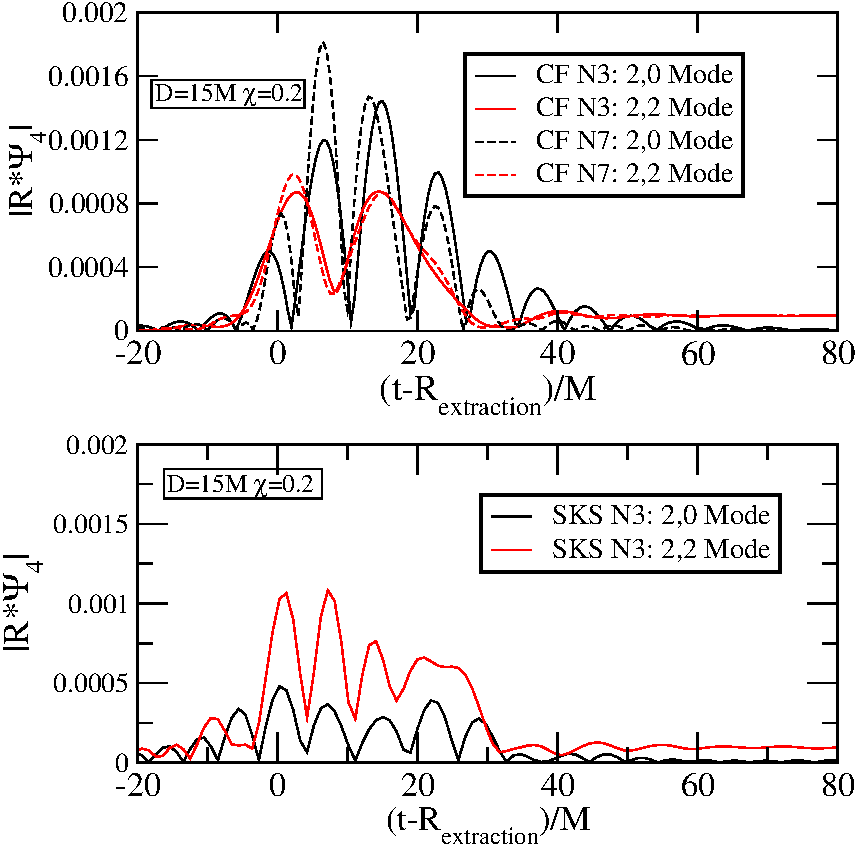
\includegraphics[scale=0.95]{chap5/HighResComparison}
  \caption[Junk radiation profiles for CF and SKS initial data, and a
  comparison to high resolution SKS initial data.]{{\it Top Panel:} Comparison of the junk radiation profiles for our usual
    highest resolution (N3) and an additional run at very highest
    resolution (N7). We see, especially for the $(2,0)$ mode, that the
    maximum peak of the junk radiation is much higher for N7, but
    additional peaks are comparable or higher for N3. \newline {\it
      Bottom Panel:} Junk radiation profile for an SKS run with the
    same parameters as in the top panel. The waveform is significantly
    different in structure from the CF waveform.
}
  \label{fig:HighResComparison}
\end{figure}

As a more robust quantity that incorporates the whole waveform, and is
less resolution dependent than $\max{|R\Psi_4^{lm}|}$, we look at the
total energy carried away from the system by gravitational waves. The
 gravitational wave energy flux is(~\cite{Boyle:2008})
\begin{equation}
F(t) =\frac{1}{16\pi}\sum_{l,m}\dot{h}_{lm}^2(t),
\end{equation}
where
\begin{equation}
\dot{h}_{lm}(t)=\int_{t_0}^{t}{\Psi_4^{lm}(t')dt'} + H_{lm}.
\end{equation}
The $H_{lm}$ are integration constants.  To measure the
  initial pulse of radiation, we use $t_0=0$ and $H_{lm}=0$.  The energy flux, $F(t)$, is shown in
the red curves in Fig.~\ref{fig:FluxSample} for conformally flat initial data (top
panel) and SKS initial data (bottom panel).  The initial burst
  is apparent in these figures; at late times $t_R\gtrsim 40M$, $F(t)$
  approaches the nearly constant energy flux of the astrophysical
  inspiral.  We are now faced with two problems: We would like to
  isolate the energy carried in junk-radiation from the energy-flux
  astrophysical inspiral.  And, we would like to do so in a robust way, 
independent of arbitrary choices.  We
  proceed as follows:

  First, we assume that the astrophysical energy flux begins at a time
  $t_{22}$, i.e.
\begin{equation}
  F_{22}(t) = F_0\,\theta(t-t_{22}).
\end{equation}
Here, $F_0$ represents the value of $F(t)$ after the pulse of
junk-radiation and $\theta$ represents the step-function.
The choice of a constant value $F_0$ is reasonable since the
timescale on which $F_{22}$ changes significantly is much longer than
the junk radiation timescale.  This energy flux is indicated by the blue dashed curves in Fig.~\ref{fig:FluxSample}.
We will
discuss our choice for $t_{22}$ shortly.  The energy in the
junk-radiation is given by
\begin{equation}\label{eq:EJ}
E_J=\int_0^{t_C}\big[(F(t)-F_{22}(t)\big]dt,
\end{equation}
where the cut-off time $t_C$ is chosen after the junk radiation has
decayed, i.e. $t_C-R\gtrsim 50M$.  The energy attributed to the junk
radiation is thus the shaded area in Fig.~\ref{fig:FluxSample}.  As
already apparent from Fig.~\ref{fig:FluxSample}, the precise value of
$t_C$ is not extremely important, because at late times $F(t)-F_{22}(t)\approx 0$.  

It remains to chose a prescription for the choice of $t_{22}$, the
time when we deem the astrophysical waveform to ``turn on''.
% In finding the total energy in junk radiation, however, it cannot
% be assumed that all the energy emitted up to $t=t_C$ is due to junk
% radiation. The astrophysical $2,2$ mode signal, $F_{22}(t)$, should
% still be present, with the junk radiation signal superimposed on
% it. The energy in junk radiation is thus written as
% \begin{equation}
% E_J=\int_0^{t_C}\left(F(t)-F_{22}(t)dt\right)
% \end{equation}
% This quantity is represented by the shaded area in
% figure~\ref{fig:FluxSample}. We choose a simple model for $F_{22}(t)$:
% $F_{22}$ turns on at some time $t_{22}$ and takes on the constant
% value of $F_0=F(t_C)$. That is,
% \begin{equation}
% F_{22}(t)=F_0\theta\left(t-t_{22}\right)
% \end{equation}
% This is represented by the blue curves in
% figure~\ref{fig:FluxSample}. 
%The choice of a constant value for the flux is reasonable since the
%timescale on which $F_{22}$ changes significantly is much longer than
%the junk radiation timescale. 
%There is no a priori way to precisely
%determine where $t_{22}$ should be. 
A simple method would be to choose
$t_{22}$ to correspond to $\max\{F(t)\}$. This seems reasonable for
the conformally flat curve in Fig.~\ref{fig:FluxSample}, but the
more wide double-peaked structure of the SKS curve shows that another
approach is needed. Instead we take $t_{22}$ to correspond to the flux
weighted centre of the junk radiation waveform. The first moment of
$F(t)-F_{22}(t)$, in other words. So,
\begin{equation}\label{eq:t22}
t_{22}=\frac{\int_0^{t_C}{t\left(F\left(t\right)-F_0\theta\left(t-t_{22}\right)\right)dt}}{\int_0^{t_C}{\left(F\left(t\right)-F_0\theta\left(t-t_{22}\right)\right)dt}}.
\end{equation}
This equation must be solved iteratively for $t_{22}$.

\begin{figure}
 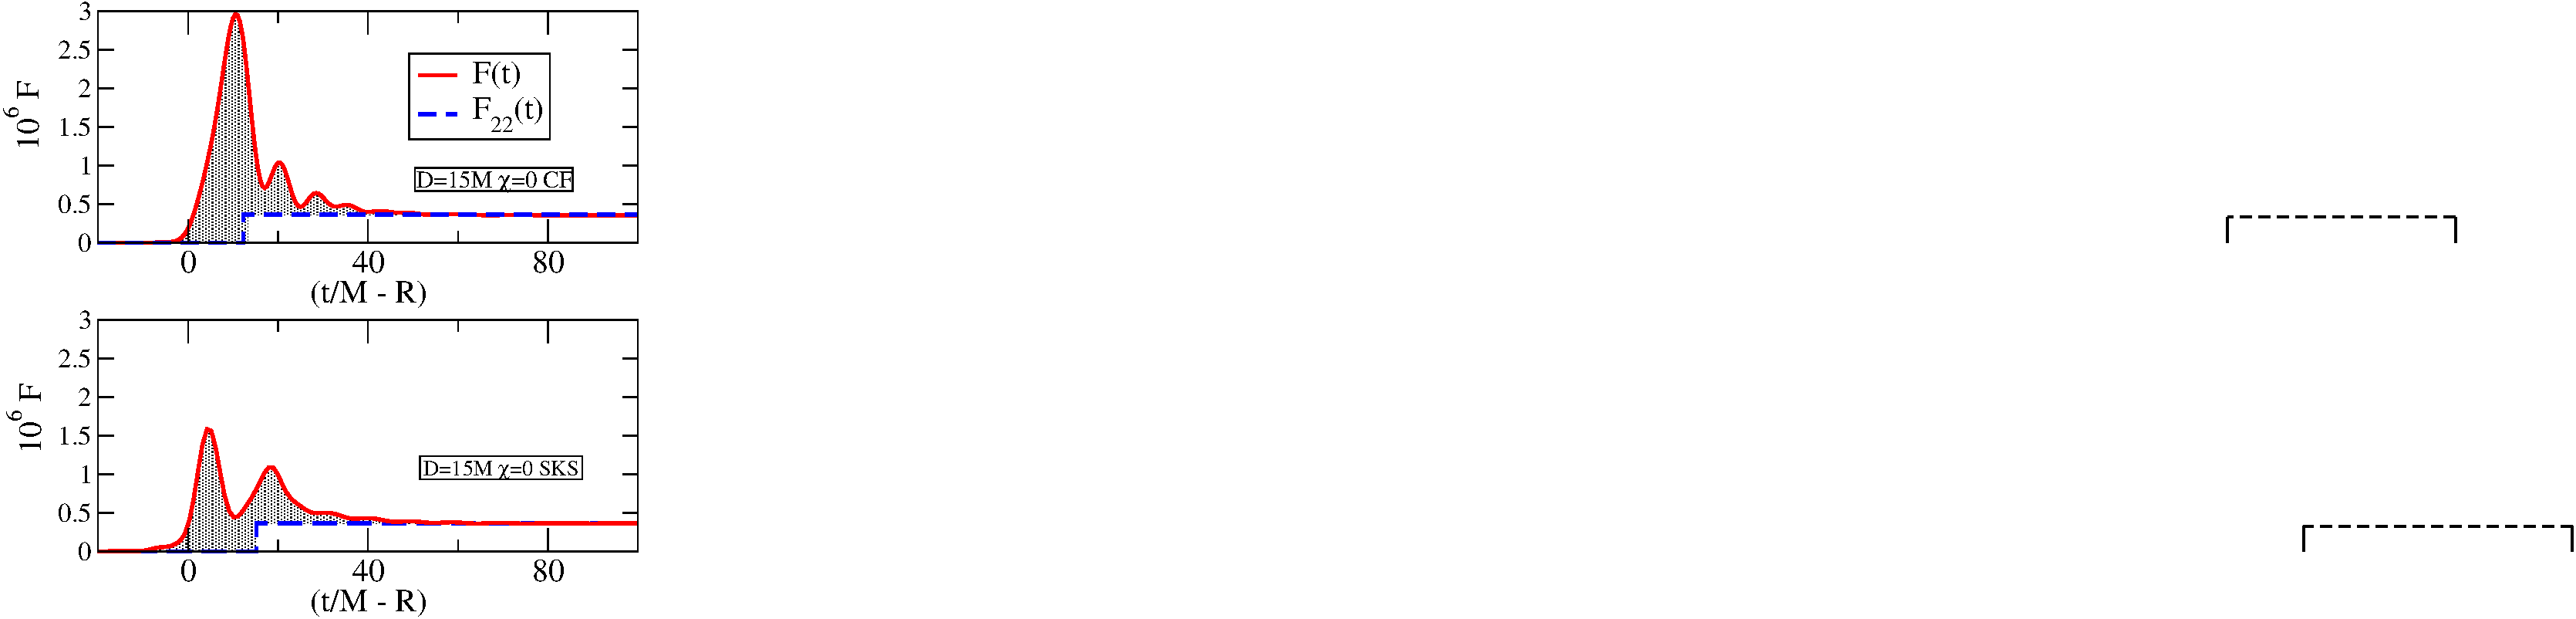
\includegraphics[scale=0.95]{chap5/FluxSample}
  \caption[The flux, $F(t)$, and the computation of $E_J$ for CF and
  SKS intitial data.]{The flux $F(t)$ is plotted for two different runs, both
    with parameters $D=15M$ and $\chi=0$. Conformally flat initial
    data is in the top panel and SKS initial data is in the bottom
    panel. The solid red curve represents the total flux, $F(t)$. The
    dashed blue curve represents $F_{22}(t)$, the astrophysical flux
    that we subtract from $F(t)$. The shaded area between the two
    curves is the energy in junk radiation, $E_J$.
}
  \label{fig:FluxSample}
\end{figure}

\subsection{Uncertainty in $E_J$}
\label{subsec:ErrorEstimation}

%\subsubsection{Resolution of the Waveform}

Several effects may influence the quantity $E_J$ computed by
  Eqs.~(\ref{eq:EJ}) and~(\ref{eq:t22}).  {\it Numerical truncation
    error} can be estimated by performing the simulations with
  different numerical resolution.  Our simulations show that in general,
  $E_J$ increases with resolution. This is because junk radiation is
a short wavelength feature, so greater resolution allows for more of
the features present to be captured.  To estimate the
uncertainty in $E_J$, we compare our $D=15M$,
$\chi=0.2$ runs at N3 and N7, as discussed earlier. We find that
at N7, $E_J$ is about $13\%$ greater than at N3. Since we don't
have such high resolutions runs available for each of our cases, we
assume that we can use this same $13\%$ difference for each of our
runs. This also assumes that at N7 the junk
radiation is nearly fully resolved, so that this difference is a good
indication of the true value. Finally, we use this same uncertainty of
$13\%$ for the SKS runs as well - while the technology is different
for the SKS runs, it should still be a reasonably good estimate, and
likely a conservative estimate, of the numerical truncation error in them.

%\subsubsection{Choice of $t_C$}

A second uncertainty arises through the {\it choice of $t_C$}.
This number is chosen manually for
each run, introducing a
  subjective element into the analysis. Examining the flux curves in
Fig.~\ref{fig:FluxSample}, for example, $t_C$ could conceivably be
chosen differently by $\sim 10 M$ and still be a
reasonable choice. {Our definition Eq.~(\ref{eq:EJ}) was meant
to be robust to small changes in $t_C$.  For $E_J$ to be a robust measurement, it should
therefore not change significantly in response to changes $\delta t_C$
that are of that order. Indeed, this is enforced by our definition of
$E_J$, which subtracts out the additional flux in the astrophysical
$(2,2)$ mode.}  To verify this assertion, we compute $E_J$ with $t_C$ in Eq.~(\ref{eq:EJ}) replaced by $t_C+\delta t_C$.  Figure~\ref{fig:EvsDtC} shows that indeed $E_J$ is almost independent of $\delta t_C$.  
%The uncertainty introduced by $t_C$ is about $1\%$. 
In Fig.~\ref{fig:EvsDtC}, $E_J$ is plotted against $t_C$
in the representative $D=15M$, $\chi=0$ case.
For each run we define a fractional
error parameter due to the choice of $t_C$, where we average the
differences for $\delta t_C = -10M$ and $\delta t_C = 10M$:
\begin{equation}
\frac{\Delta E}{E} = \frac{|E(t_C+10M) - E(t_C)| + |E(t_C) - E(t_C -
  10M)|}{2E(t_C)}
\end{equation}
This uncertainty ranges from $\sim 0.25\%$ to $\sim 3.75\%$ throughout
all of ours runs.

\begin{figure}
 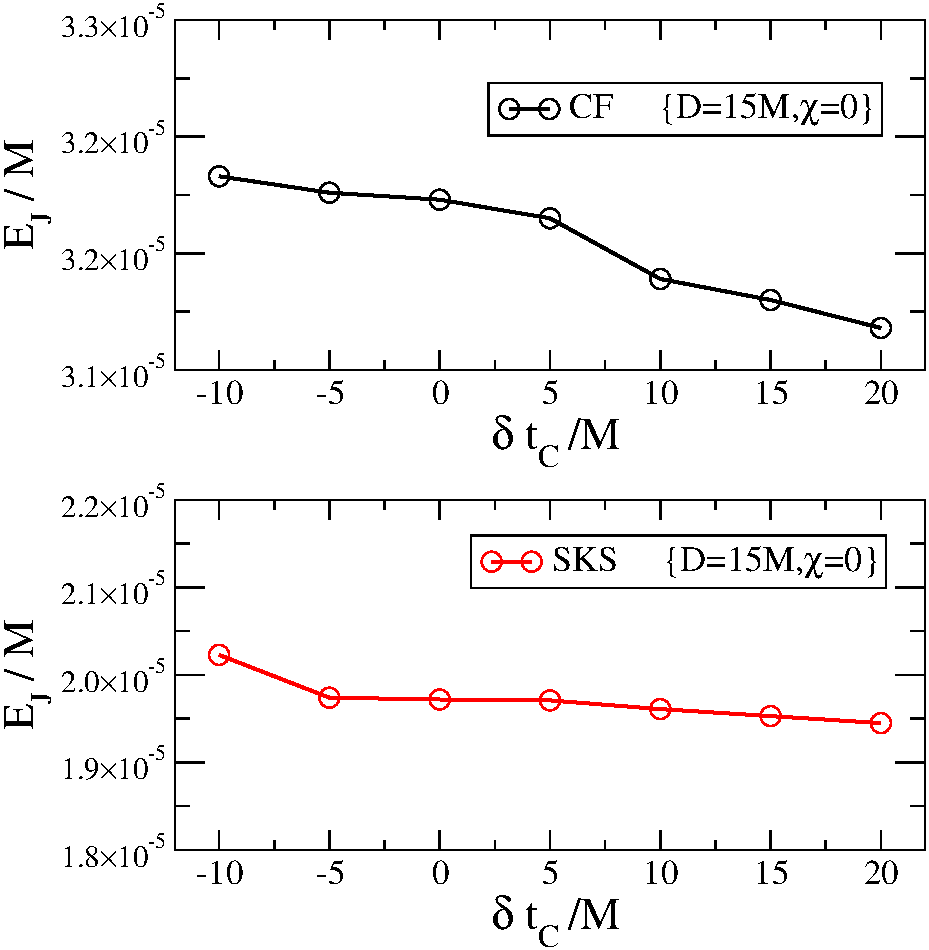
\includegraphics[width=0.95\columnwidth]{chap5/EvsDtj}
  \caption[$E_J$ as a function of $\delta t_C$.]{$E_J$ is plotted against $\delta t_C$, representing changes
    to the selected value of $t_C$ for runs where $D=15M$,
    $\chi=0$. The results for conformally flat initial data are shown
    in the top panel, and SKS initial data in the bottom
    panel. Typical changes in $E_J$ are on the order of a few
    percent.}
 \label{fig:EvsDtC}
\end{figure}


A third error in $E_J$ arises through {\it the finite radius
    of gravitational wave extraction}.  In this study, gravitational waves are extracted at radii $R_{\rm ex}\sim 300-400M$.  Gravitational waves extracted at finite radii are subject to near-field effects which may cause the extracted
waveforms to differ from the one that would be observed at
infinity.  
To estimate the error in $E_J$ due to the finite extraction radius, we
use the following procedure. For each of our runs, we take $E_J$ at
several extraction radii, and examine $E_J$ as a function of
$1/R_{ex}$. We then extrapolate
\begin{equation}
E_{\infty} = \lim_{1/R_{ex}\rightarrow 0}E_J(1/R_{\rm ex})
\end{equation}
using a linear fit in $1/R_{\rm ex}$ to estimate the behaviour of $E_J$ at infinity. We
then take the fractional difference
\begin{equation}
\frac{\Delta E}{E} = \frac{E_{\infty}-E_J}{E_J}
\end{equation}
as our error estimate. This parameter is on the order of $10\%$ for
most of our runs. Note, however, that we still use $E_J$ and not $E_{\infty}$ as
our measure of energy in the pulse. In Fig.~\ref{fig:EvsRextr} we illustrate an
example of this procedure, plotting $E_J$ vs. $1/R_{ex}$ for one case,
$D=15M, \chi=0$, for both CF and SKS data.

\begin{figure}
  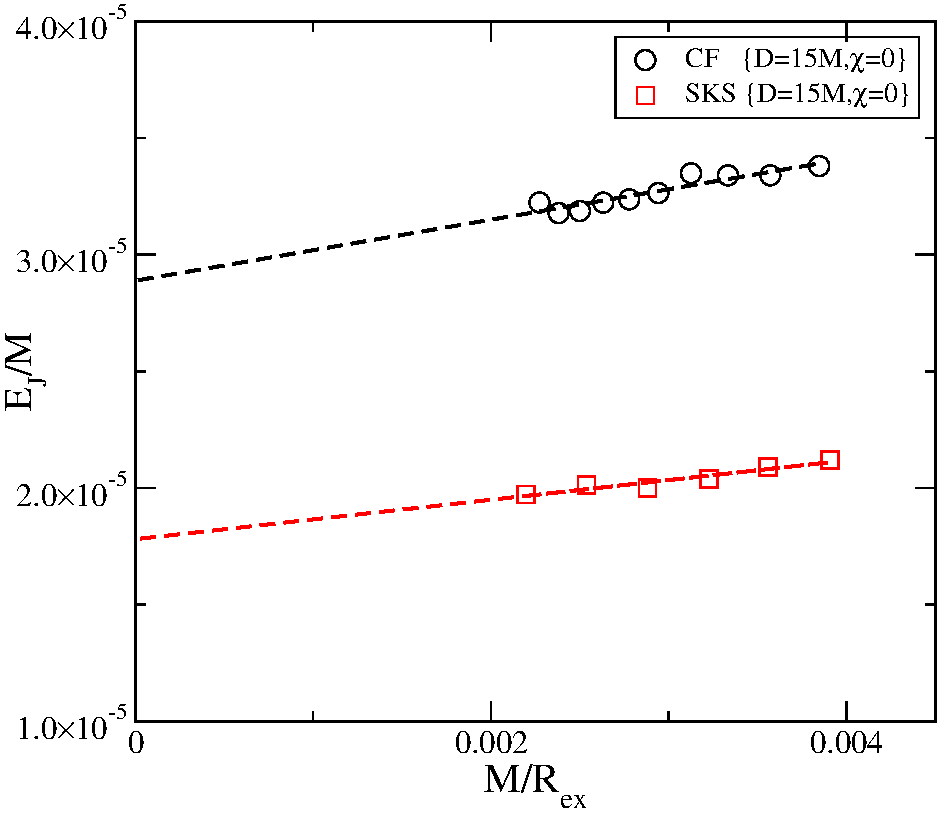
\includegraphics[scale=0.95]{chap5/EvsRextr}
  \caption[$E_J$ as a function of $1_R/{\rm ex}$.]{$E_J$ as a function of $1/R_{ex}$, where $R_{ex}$ is the
    extraction radius. This is for the case where $D=15M$, $\chi=0$,
    with CF initial data in the left panel and SKS initial data in the
    right panel. The extrapolation
    to $1/R_{ex}\rightarrow 0$ allows us to estimate the error on
    $E_J$ due to finite extraction radius effects. }

  \label{fig:EvsRextr}
\end{figure}

A final factor that could influence the estimated $E_J$ is the
{\it eccentricity of the orbit of the black holes}. Previously we argued
that it is important for astrophysically realistic binaries to have
low eccentricity. We now consider how it affects the junk radiation, specifically the effect on $E_J$. We examine the case $D=25M \chi=0.1$
for CF data, as this particular case led to a fairly large range of
eccentricities in the reduction process;
$e\sim\{0.03,0.008,0.0006\}$. The measured $E_J$ for these three cases
is $10^6E_J=\{7.053\pm0.38\%, 7.204\pm0.53\%, 7.174\pm0.58\%\}$. Here,
the quoted uncertainty is purely due to the choice of $t_C$. The
differences between the first two eccentricities is $2.10\%$ and it is
$0.42\%$ for the last two. Because the latter difference is less than
the uncertainty due to the choice of $t_C$, the two runs are
effectively indistinguishable, and we conclude that we can safely
ignore the effects of residual eccentricity once we have $e\lesssim
0.008$. However, to be ``safe'', we have generally reduced the
eccentricity of all of our runs to $e\lesssim 0.002$.

%\harald{A final factor influencing the estimated $E_J$ is the
%{\em eccentricity of the orbit of the black holes}. }
%\subsubsection{Effect of Eccentricity}
%\label{subsec:EccentricityEffect}
%\red{[As discussed: Remove Fig.~\ref{fig:EccComparison}, state here in main-text $E_J$ for the different eccentricities, conclude that the effect of eccentricity is below xxx.  Also shorten text, by removing unneeded words and information] }
%Previously, we argued that it is important for astrophysically
%realistic binaries to have low eccentricity. We now examine how
%eccentricity actually affects the junk radiation. In
%figure~\ref{fig:EccComparison}, we have plotted the leading order (2,0) mode
%of the junk radiation for eccentricities of $e\approx
%\{0.03,0.008,0.0006\}$. This was done for runs where $D=25M$,
%$\chi=0.1$, and at medium resolution, i.e. Lev2. This was chosen as it
%happened to give us the largest range of eccentricities available, and
%often the highest resolution Lev3 runs at higher eccentricity were
%terminated earlier. We find that the junk radiation amplitude is
%nearly independent of the eccentricity. Figure ~\ref{fig:EccComparison} shows
%that there is some visible difference between
  %$e\approx 0.03$ and $e\approx 0.008$, but nearly no difference
  %between $e\approx 0.008$ and $e\approx 0.0006$.  The impact of eccentricity
%on the junk-radiation is even smaller for the $(2,2)$
  %mode. Figure~\ref{fig:EccComparison} essentially shows that we can
  %safely ignore the effects of residual eccentricity once we have $e
  %\lesssim 0.008$. However, to be ``safe'', we have generally reduced
  %the eccentricity of all of our runs to $e\lesssim 0.002$.
%\begin{figure}
%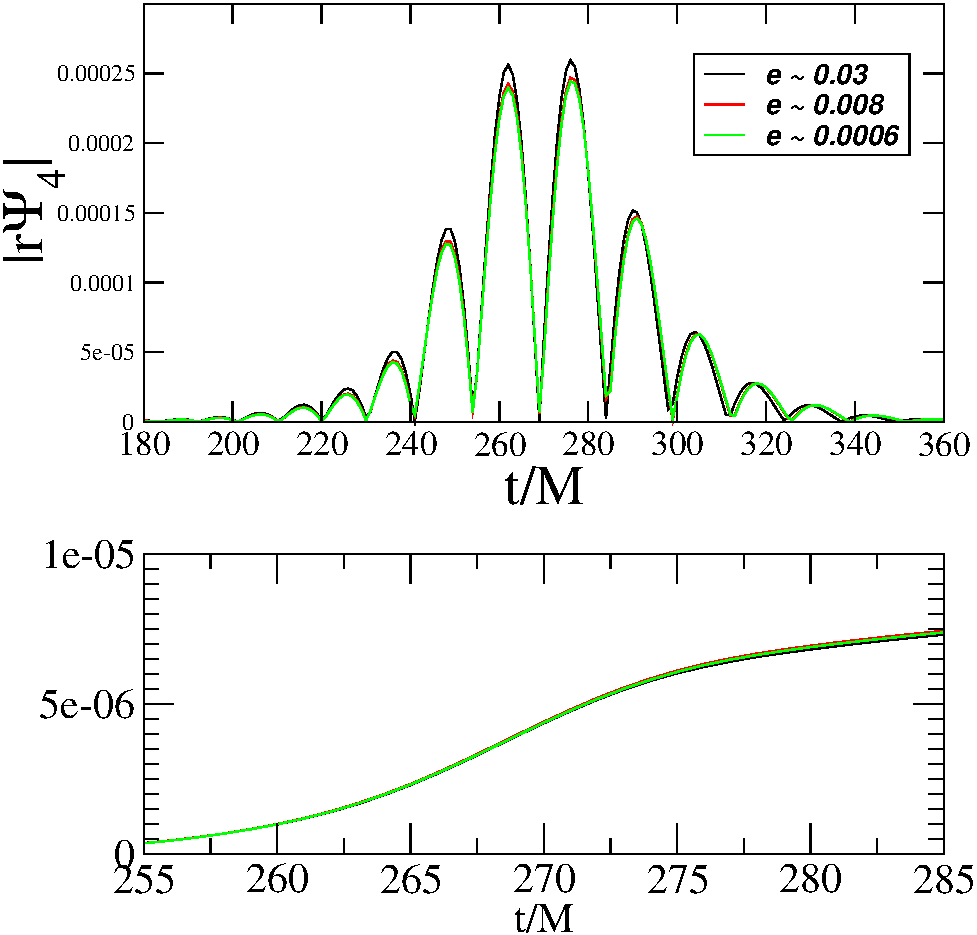
\includegraphics[scale=0.5]{EccComparison}
 % \caption{\note{Kill this plot, and add words describing it to the text}\note{Define what is plotted.  If this is the integral of
%      $\dot h_{20}^2$, then wouldn't it be more suitable to plot
 %     $E(t)$ directly at different resolutions?  Include legend} A
   % comparison of the $2,0$ mode of junk radiation at three different
   % eccentricities. At the two lowest eccentricities, the junk
   % radiation profiles are essentially the same, telling us that we
   % can effectively ignore eccentricities under $e \sim
   % 0.008$}
 % \label{fig:EccComparison}
%\end{figure}

\subsection{Transient behaviour in Black Hole quantities}

\subsubsection{Mass Increase}
Besides the energy carried away in junk radiation, we utilize two further
diagnostics of transients arising from imperfect initial data.
The first diagnostic is the irreducible
mass of the black hole, $M_{irr} = \sqrt{A/(16\pi)}$, where $A$
is the area of the black hole's apparent horizon. 
In the first few $M$ during the evolution, the apparent horizon mass
$M_{\rm irr}(t)$ increases by a small amount, before settling down to
an approximately constant value. This effect is easily apparent for CF initial data plotted in the upper panel of Fig.~\ref{fig:MassIncreaseCFSKS}.
We characterize the increase in mass due to initial transients by 
\begin{equation}
\delta M(t)=\frac{M_{irr}(t)}{M_{irr}(0)}-1
\end{equation}
and the equilibrium parameter $\delta M_{eq} = \delta M(t_{\rm eq})$.
Here $t_{\rm eq}$ is a time where the mass-increase is complete, and
levels off; typically $\sim20M$. 

For SKS initial data the behaviour of $M_{\rm irr}(t)$ is more
  complex.  Within the first few $M$, $M_{\rm irr}(t)$ shows a rapid,
  albeit small increase, presumably due to relaxation of the geometry
  in the immediate vicinity of the black holes.  The trend here is
  similar to the CF initial data, in that larger spins result in a
  larger increase of $M_{\rm irr}(t)$, albeit the magnitude of the
  increase is about a factor 50 smaller for SKS initial data.
  Subsequently, starting at $t\sim 40M$, the SKS-runs show a second
  set of features, oscillations with amplitude $\sim 2\times 10^{-5}$ lasting about
  $60M$.  The features of these oscillations are similar to each other even for runs with different spin $\chi$.  Therefore, it is
  likely that these oscillations are caused by features in the initial
  data set {\it away} from the black holes.

In Fig.~\ref{fig:MassIncreaseCFSKS}, curves of $M_{irr}(t)$ are
shown at different spins, at constant $D=15M$, with Conformally flat
initial data in the top panel, and SKS initial data in the bottom
panel. There is a clear qualitative between the CF and SKS curves. The CF data evidently forms a increasing sequence of $\delta_M$ with
$\chi$, and $\delta_M$ is clearly well-defined in each case. However,
the SKS data exhibits oscillatory behaviour that is relatively spin
independent, and there is not a clear way to define $\delta_M$. The
scale of the oscillations is on the order of $10^{-5}$. Our conclusion
is that these are numerical oscillations and the contribution from
junk radiation is not directly measurable, and we do not seek to
characterize their parameter space dependence any further.

\begin{figure}
 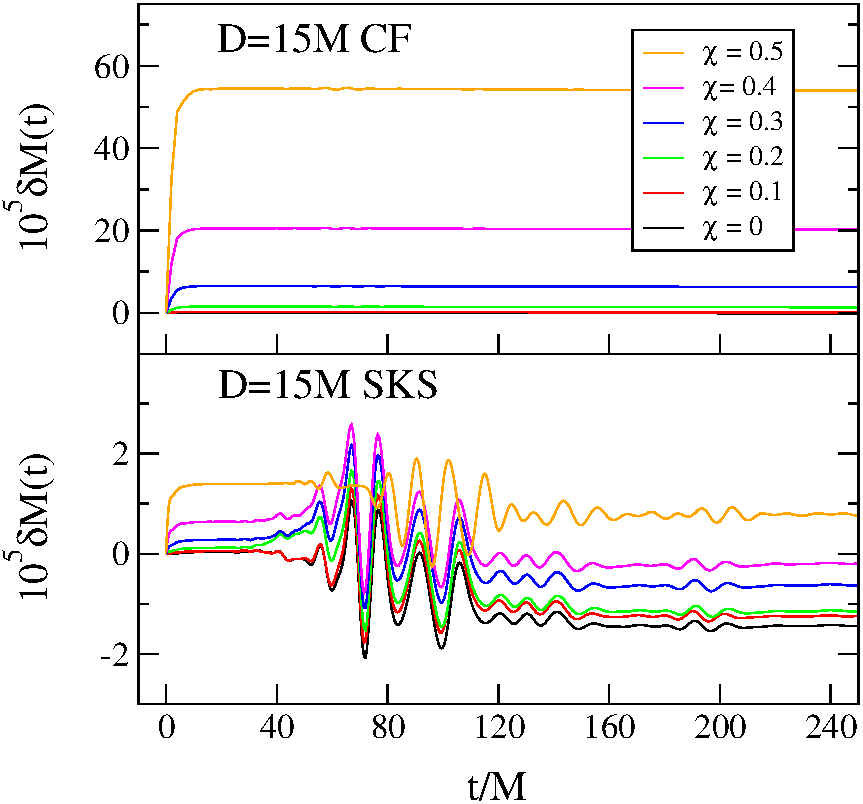
\includegraphics[width=0.95\columnwidth]{chap5/MassIncreaseCFSKS}
  \caption[Normalized irreducible mass curves for CF and SKS data.]{Normalized irreducible mass curves for CF data (top panel)
    and SKS data (bottom panel) for all of the different spins in the
    covered parameter space and $D=15M$ remaining constant. }
  \label{fig:MassIncreaseCFSKS}
\end{figure}

Figures~\ref{fig:CFMConvergence1} and~\ref{fig:SKSMConvergence1} show
convergence tests for one of the spin-values shown in
Fig.~\ref{fig:MassIncreaseCFSKS}.  ($D=15M$, $\chi=0.3$).  The top
panels of Figs.~\ref{fig:CFMConvergence1}
and~\ref{fig:SKSMConvergence1} show $M_{\rm irr}(t)$ of one black hole
computed at different numerical resolutions, and the bottom panels
show differences in $M_{\rm irr}(t)$ computed at neighbouring
resolutions.  Note that our parameter space studies presented in
Sec.~\ref{sec:Results} were usually performed on resolution ``N3''; we
have run ``N4'' only for select cases to test convergence.  The CF
initial data shows rapid convergence and the features in the upper
panel of Fig.~\ref{fig:MassIncreaseCFSKS} are well resolved.  For the
SKS data, Fig.~\ref{fig:SKSMConvergence1} indicates convergence,
albeit much more slowly.

The magnitude of the change of $M_{\rm irr}(t)$ is much smaller for
SKS initial data than for CF initial data ($\sim 10^{-5}$ vs. $\sim
5\times 10^{-4}$).  The changes in $M_{\rm irr}(t)$ for SKS initial
data approach our numerical truncation error, and are furthermore
ambiguous due to the extra features apparent in
Fig.~\ref{fig:MassIncreaseCFSKS}.  Therefore, we shall not attempt to
quantify them in detail, beyond giving upper bounds of the change on
$M_{\rm irr}$ for SKS data.


\begin{figure}
 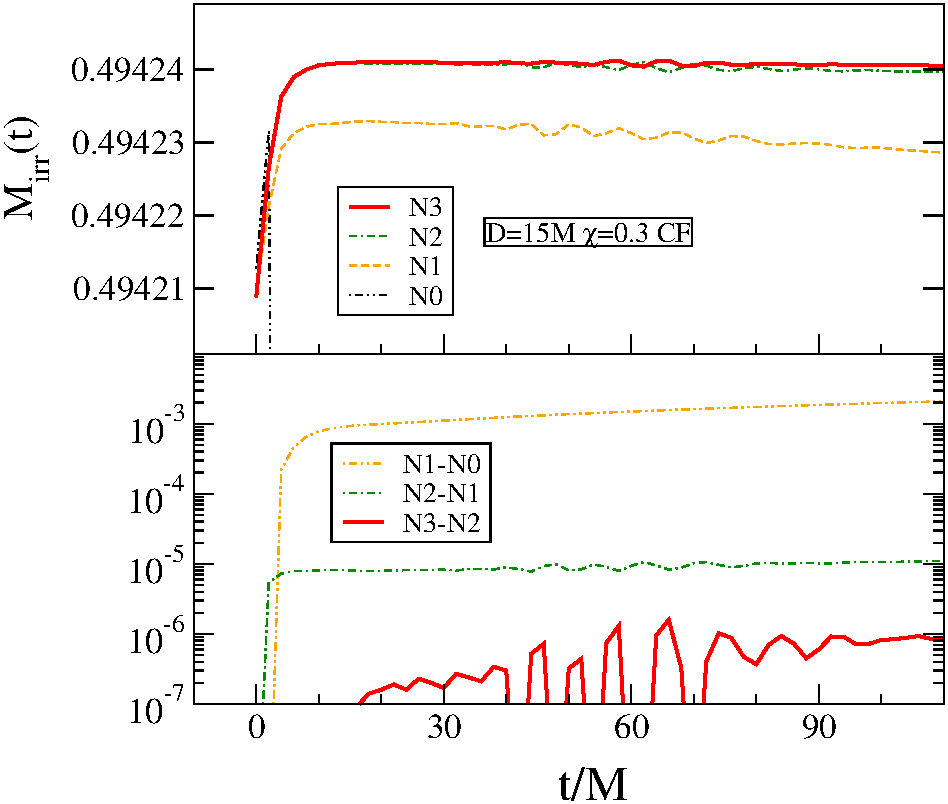
\includegraphics[scale=0.95]{chap5/CFMConvergence1}
  \caption[Convergence of $M_{\rm irr})(t)$ for CF initial data.]{Convergence test of $M_{irr}(t)$ for CF initial data in the
  case $D15=M$, $\chi=0.3$. The top panel shows $M_{irr}(t)$ at
  different resolutions, and the bottom panel shows the difference
  between consecutive resolutions.}
  \label{fig:CFMConvergence1}
\end{figure}

\begin{figure}[!htbp]
 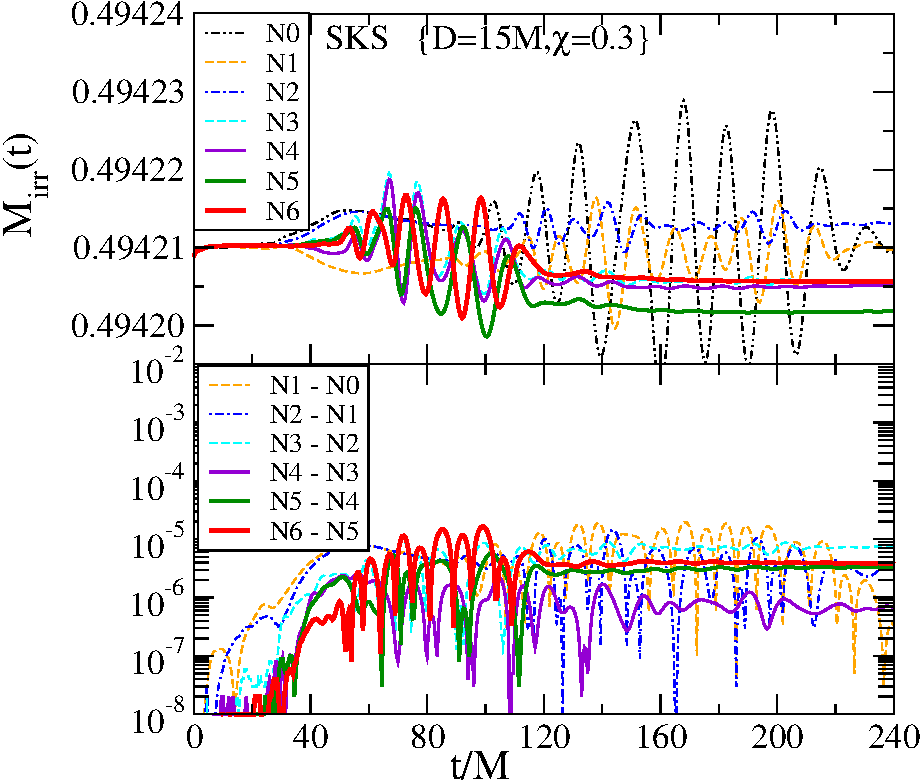
\includegraphics[scale=0.95]{chap5/SKSMConvergence1}
  \caption[Convergence of $M_{\rm irr})(t)$ for SKS initial
  data.]{Convergence test of $M_{irr}(t)$ for SKS initial data in the
  case $D15=M$, $\chi=0.3$. The top panel shows $M_{irr}(t)$ at
  different resolutions, and the bottom panel shows the difference
  between consecutive resolutions.}

  \label{fig:SKSMConvergence1}
\end{figure}

\subsubsection{Spin Decrease}

Our third and final quantification of junk radiation comes from the
black hole's spin $S(t)$. At early times in each simulation --seen in Fig.~\ref{fig:SvsT2}, the spin
of each black hole decreases and oscillates rapidly. Eventually, at
some time $t_{eq}$, the spin reaches some approximately constant
value, which is lower than the initial spin, $S(0)$. This effect can
be interpreted as angular momentum being carried away from the system
by junk radiation. Note that we use the dimension-ful quasi-local
angular momentum, measured with approximate Killing vectors as
described in~\cite{Lovelace2008}. We use $S$ rather than $\chi=S/M^2$
to de-couple the change in spin from the change in mass.

%We illustrate this effect in figure~\ref{fig:SStabilize}. Using
%representative runs where $D=15M$ and $\chi=0.5$, $S(t)/S(0)$
%is plotted for conformally flat initial data in the top panel, and SKS
%initial data in the bottom panel. It is worth noting that $S(t)$
%stabilizes on a significantly larger timescale for the SKS initial
%data, but also that it deviates significantly less from $S(0)$.

%\begin{figure}
% 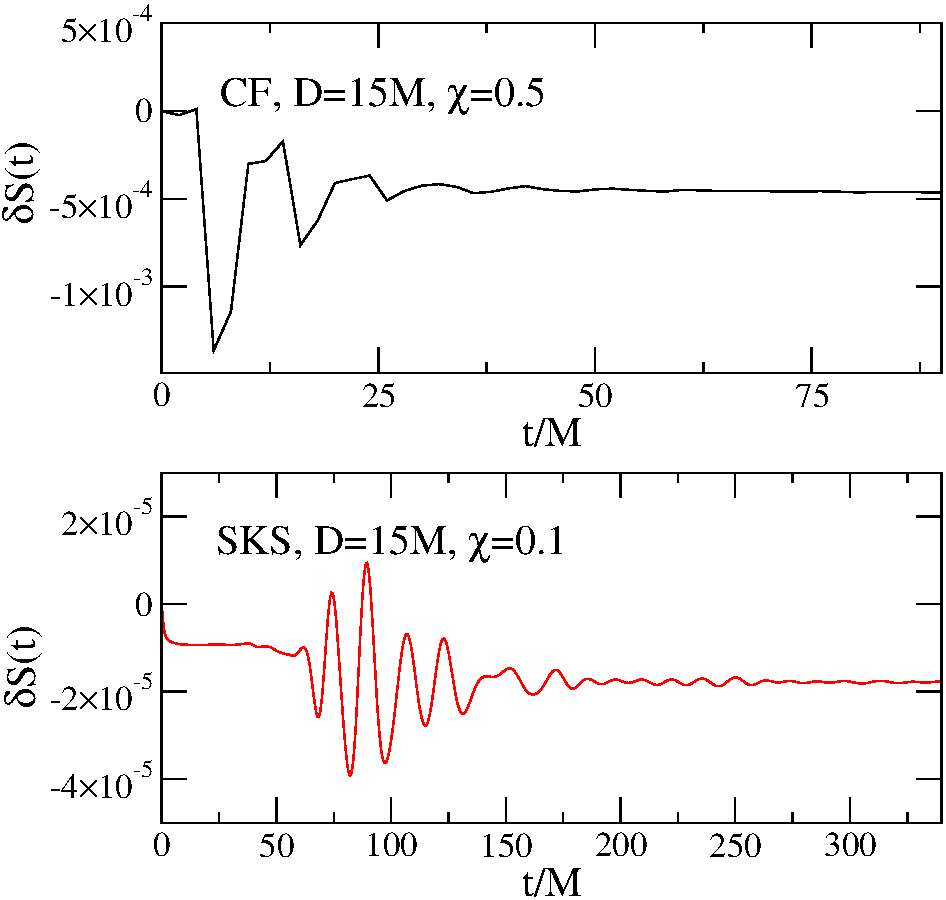
\includegraphics[scale=0.50]{SStabilize}
 % \caption{\note{Do Caption!}}
 % \label{fig:SStabilize}
%\end{figure}

%\begin{comment}
%Our third and final quantification of junk radiation comes from the
%black hole's spin $S(t)$.  This is the dimension-ful quasi-local
%angular momentum, measured with approximate Killing vectors as
%described in~\cite{Lovelace2008}.  At early times the spin $S(t)$ of
%each black hole decreases and oscillates rapidly.Eventually, at some
%time $t_{eq}$ it reaches an approximately constant value that is lower
%than the initial spin. This effect can be interpreted as angular
%momentum being carried away from the system by junk radiation. This is
%illustrated in Fig.~\ref{fig:SStabilize}, for a run with parameters
%$D=15M$, $\chi=0.5$.  Note that we use the dimensionful quasi-local
%angular momentum $S$.  We utilize $S$ rather than $\chi=S/M^2$, to
%de-couple the change in spin from the change in mass.  Fundamentally,
%we measure $S$ and $M_{\rm irr}$. 
%\end{comment}

Analogous to $\delta M(t)$, we can define the parameter $\delta S(t)$ as the
fractional spin decrease of the black hole:
\begin{equation}
\delta S(t)=\frac{S(t)}{S(0)} - 1
\end{equation}
and the equilibrium parameter $\delta S_{eq}=\delta S(t_{eq})$, where $t_{eq}$ the
time when $\delta S(t)$ has reached some nearly constant value.
In practice, we compute $\delta S_{eq}$ as the average value of
$\delta S(t)$
over some suitable interval around $t_{eq}$.

Analogous to Figs.~\ref{fig:CFMConvergence1}
and~\ref{fig:SKSMConvergence1}, Figs.~\ref{fig:CFSConvergence1} and
~\ref{fig:SKSSConvergence1} demonstrate convergence tests for $\delta
S(t)$, again for the case $D=15M, \chi=0.3$. Similar to what was see
in the convergence test for $M_{\rm irr}(t)$, the CF data convergences
rapidly, while we see no clear convergence in the SKS data going up to N6.

\begin{figure}
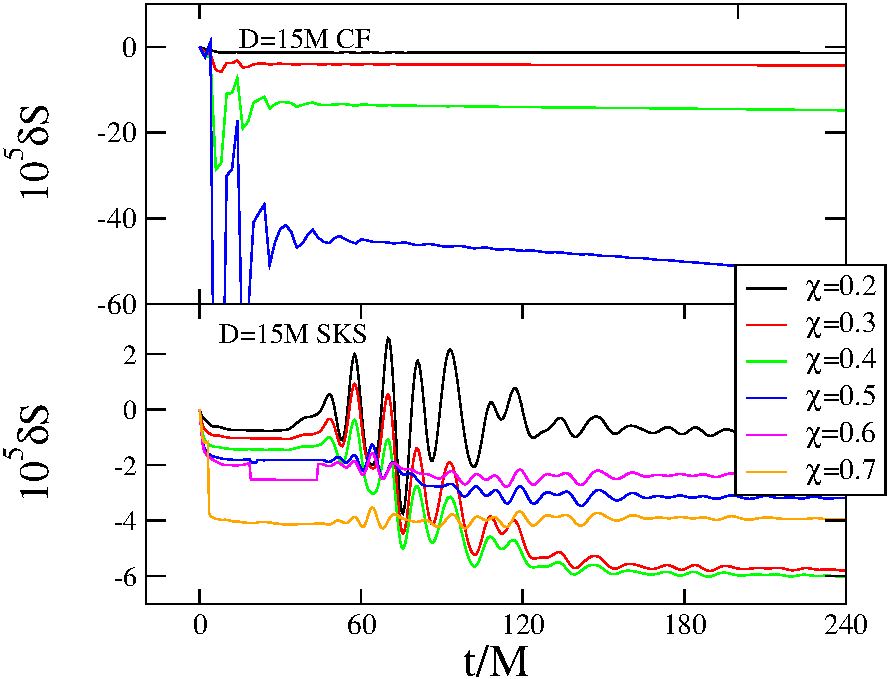
\includegraphics[width=0.95\columnwidth]{chap5/SvsT2}
\caption[$\delta S(t)$ for CF and SKS initial data.]{Fractional change in spin relative to $t=0$, $\delta S = S(t)/S(t=0)-1$.  The top panel shows conformally flat initial data and the bottom panel SKS data (note the different scale).  All simulations at distance $D=15M$.}
\label{fig:SvsT2}
\end{figure}


\begin{figure}
  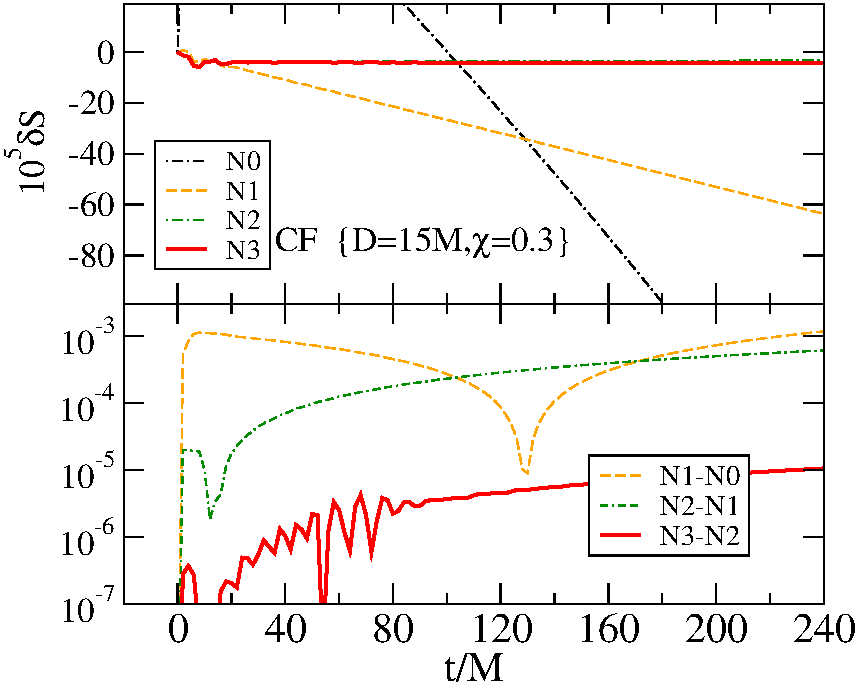
\includegraphics[width=0.95\columnwidth]{chap5/CFSConvergence1}
  \caption[Convergence test of $\delta S(t)$ for CF initial data.]{Convergence test of $\delta S(t)$ for CF initial data in the case
    $D=15M$, $\chi=0.3$. The top panel shows $\delta S(t)$ at different
    resolutions and the bottom panel shows the differences between
    consecutive resolutions}
  \label{fig:CFSConvergence1}
\end{figure}

\begin{figure}
  \includegraphics[width=0.95\columnwidth]{chap5/SKSSConvergence1}
  \caption[Convergence test of $\delta S(t)$ for SKS initial data.]{Convergence test of $\delta S(t)$ for SKS initial data in the case
    $D=15M$, $\chi=0.3$. The top panel shows $\delta S(t)$ at different
    resolutions and the bottom panel shows the differences between
    consecutive resolutions}
  \label{fig:SKSSConvergence1}
\end{figure}

%\begin{figure}
%  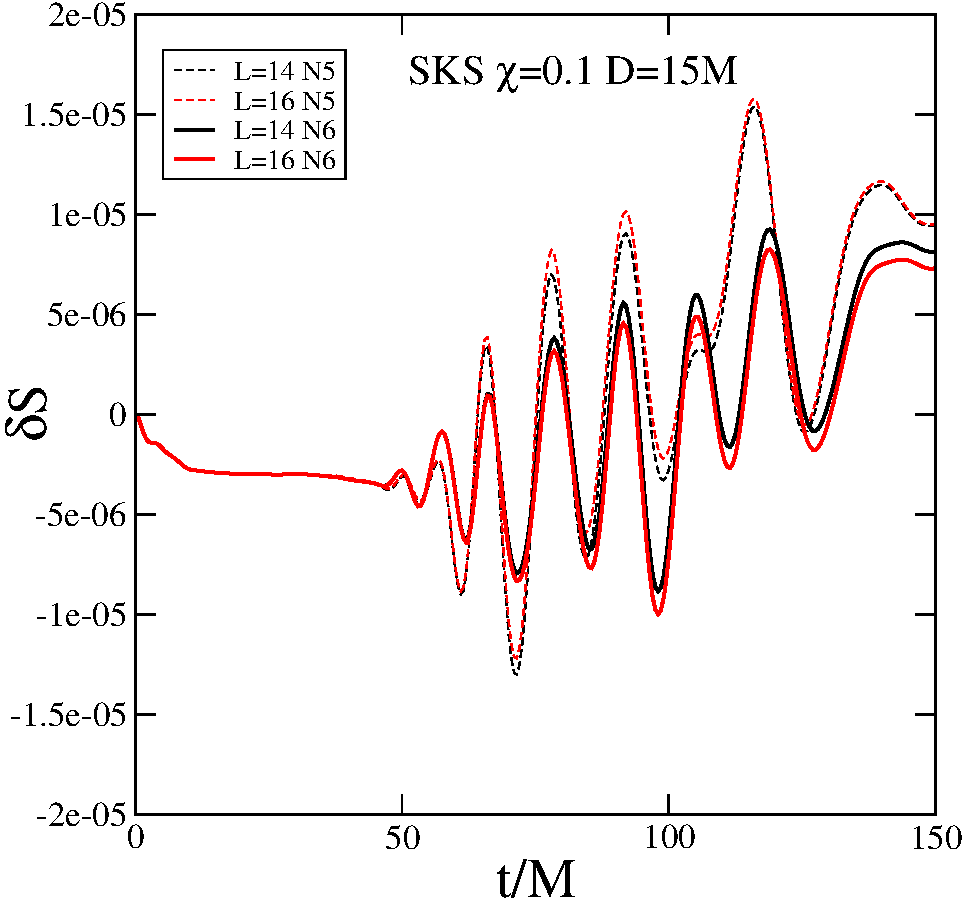
\includegraphics[width=0.95\columnwidth]{chap5/dS_SKS_S1}
%\end{figure}

%\begin{figure}
 % 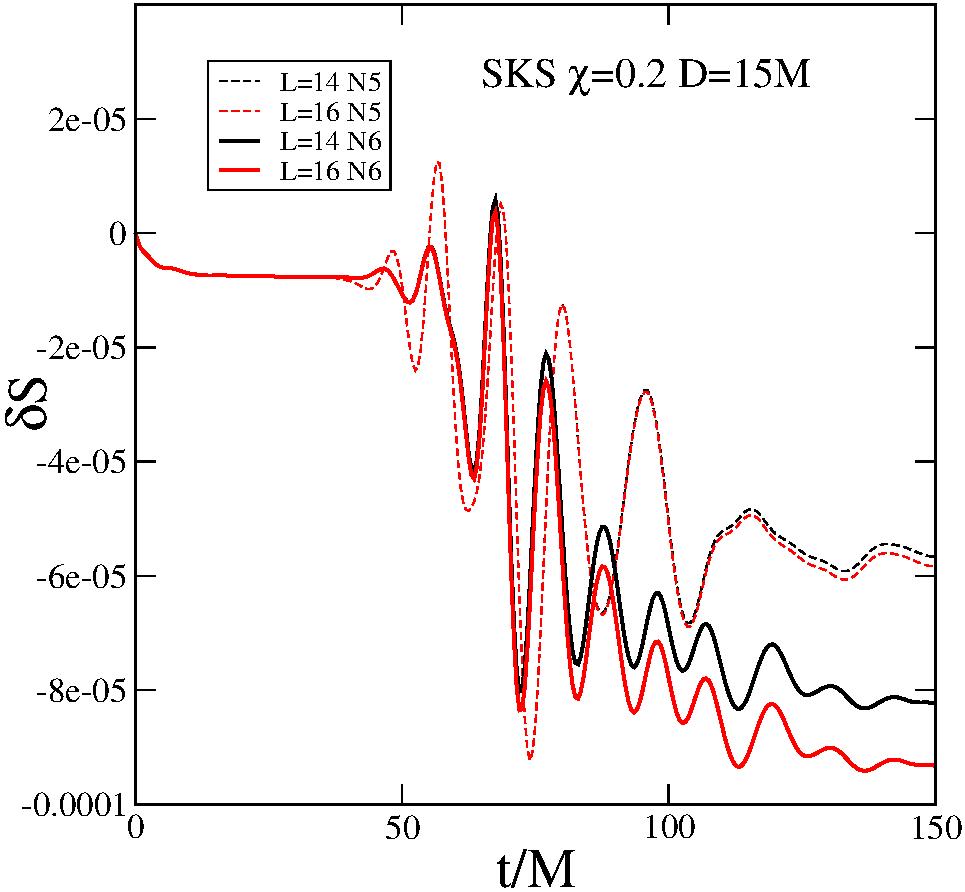
\includegraphics[width=0.95\columnwidth]{chap5/dS_SKS_S2}
%\end{figure}

%\begin{figure}
 % 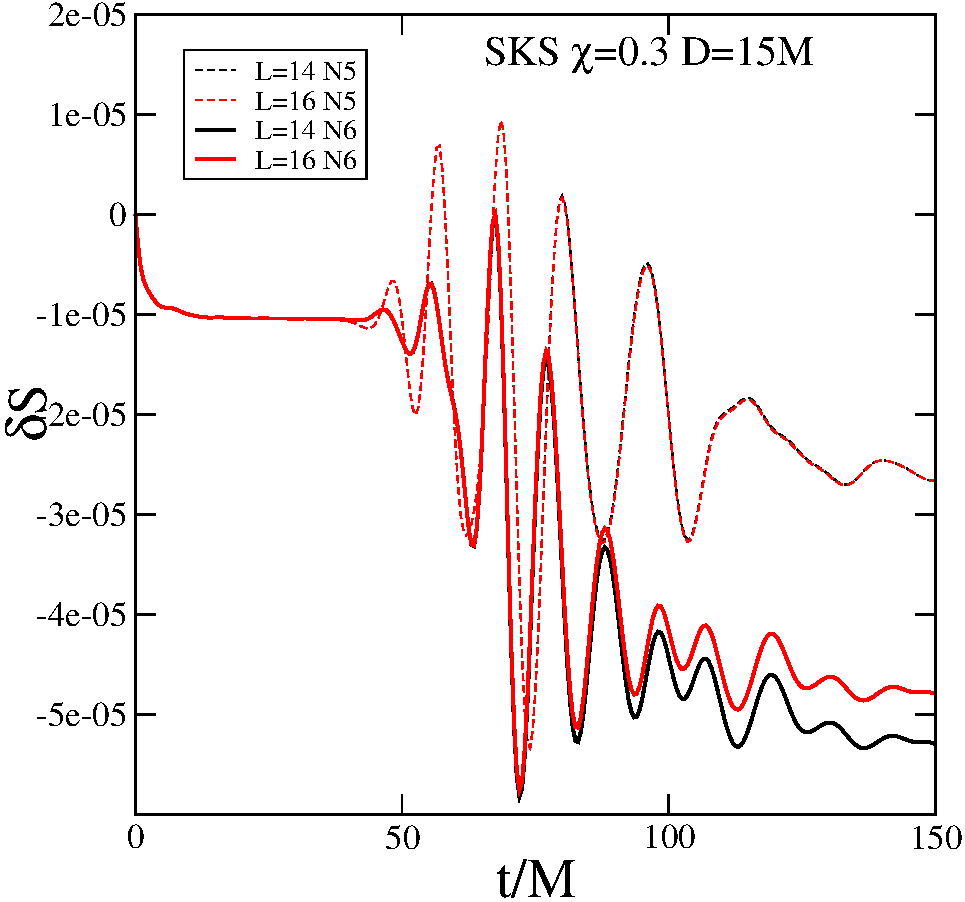
\includegraphics[width=0.95\columnwidth]{chap5/dS_SKS_S3}
%\end{figure}

%\begin{figure}
 % 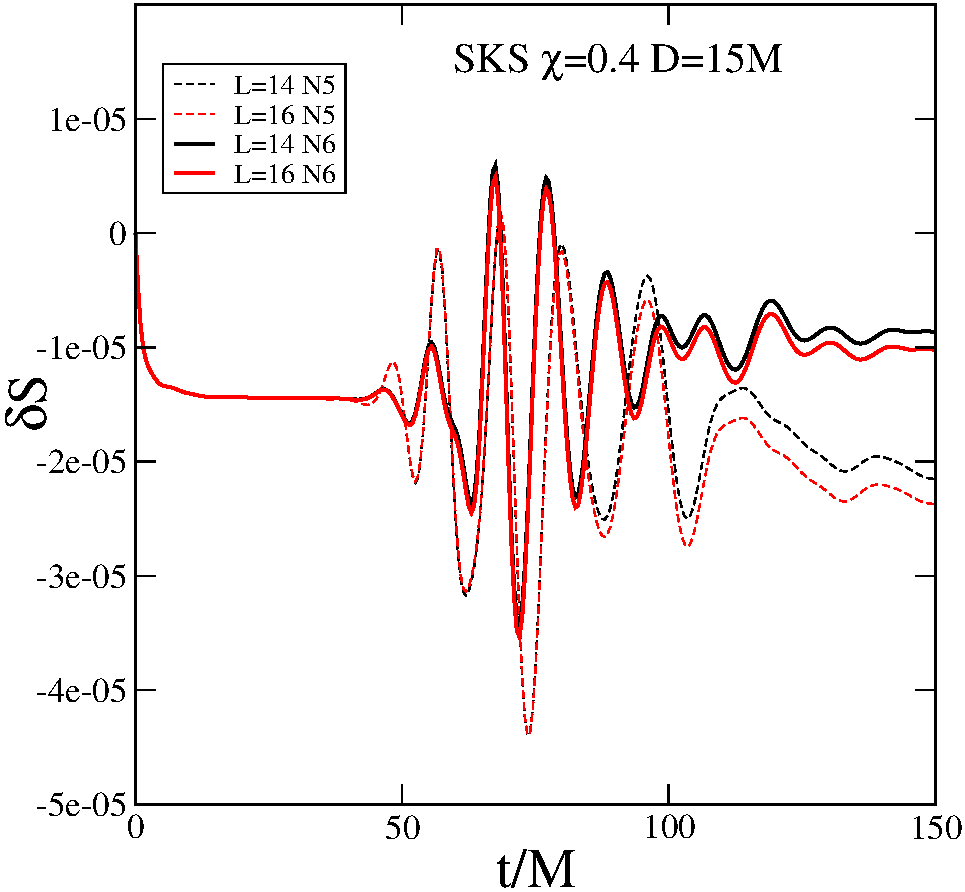
\includegraphics[width=0.95\columnwidth]{chap5/dS_SKS_S4}
%\end{figure}

%\begin{figure}
 % 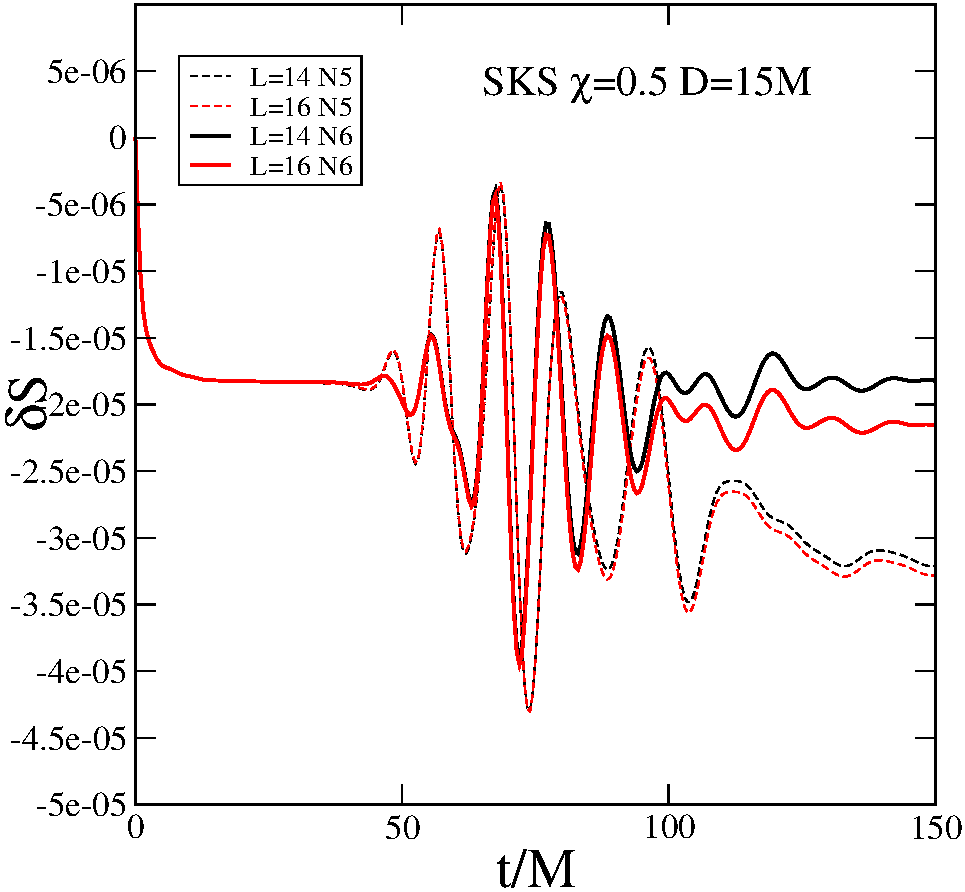
\includegraphics[width=0.95\columnwidth]{chap5/dS_SKS_S5}
%\end{figure}

%\begin{figure}
 % 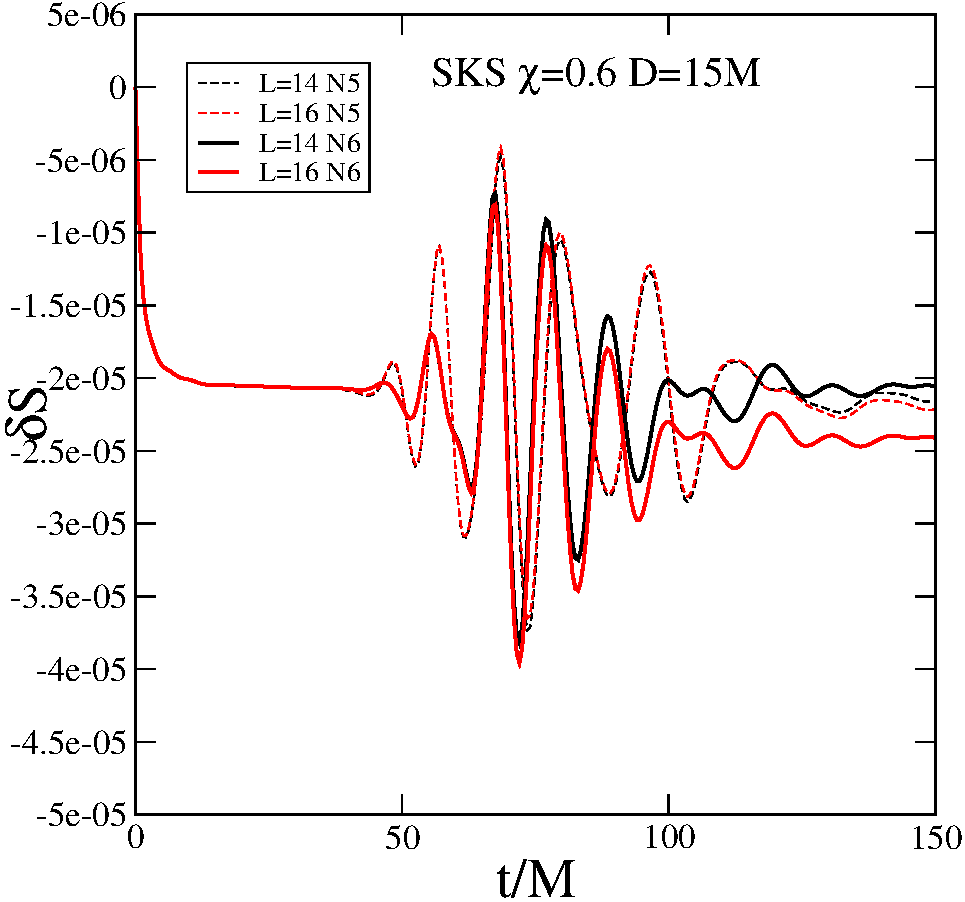
\includegraphics[width=0.95\columnwidth]{chap5/dS_SKS_S6}
%\end{figure}

%\begin{figure}
 % 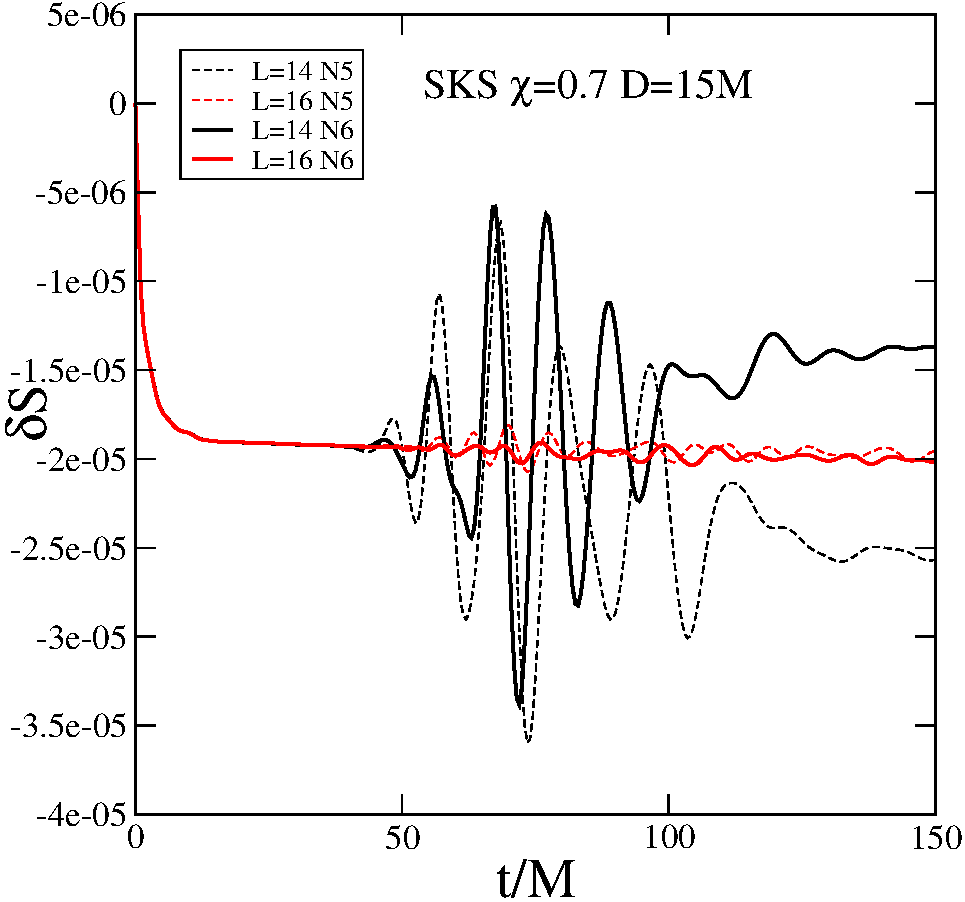
\includegraphics[width=0.95\columnwidth]{chap5/dS_SKS_S7}
%\end{figure}

%\begin{figure}
 % 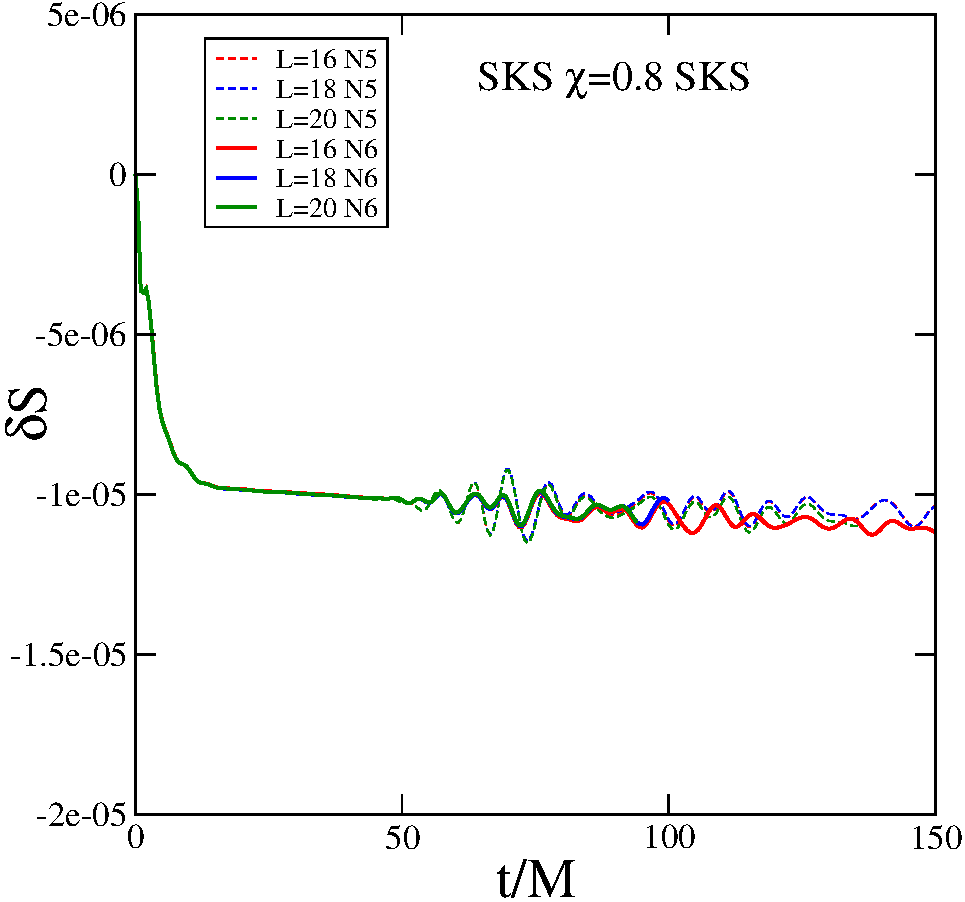
\includegraphics[width=0.95\columnwidth]{chap5/dS_SKS_S8}
%\end{figure}


%\begin{figure}
 % \includegraphics[width=0.99\columnwidth]{SKSSConvergence1}
 % \caption{Same as Fig.~\ref{fig:CFSConvergence1} but for SKS data}
 %\includegraphics[width=0.99\columnwidth]{dsConvTestS8}
 % \caption{Same as above, but $\chi=0.8$}
 % \label{fig:SKSSConvergence1}
%\end{figure}



\section{Results}
\label{sec:Results}




\subsection{Energy in Junk Radiation}

Figure~\ref{fig:EvsS} shows the energy in the pulse of junk radiation,
for all of our runs, as a function of spin. It is clear that within
the uncertainty of our simulations, $E_J$ has virtually no dependence
on the spins of the black holes. The only exception may be that for
conformally flat data, $E_J$ seems to increase as $\chi\rightarrow
0.5$. This is most visible in the $D=12M$ case. Perhaps the dependence
of $E_J$ on $\chi$ could become important for $\chi > 0.5$ if this
trend continues.

\begin{figure}
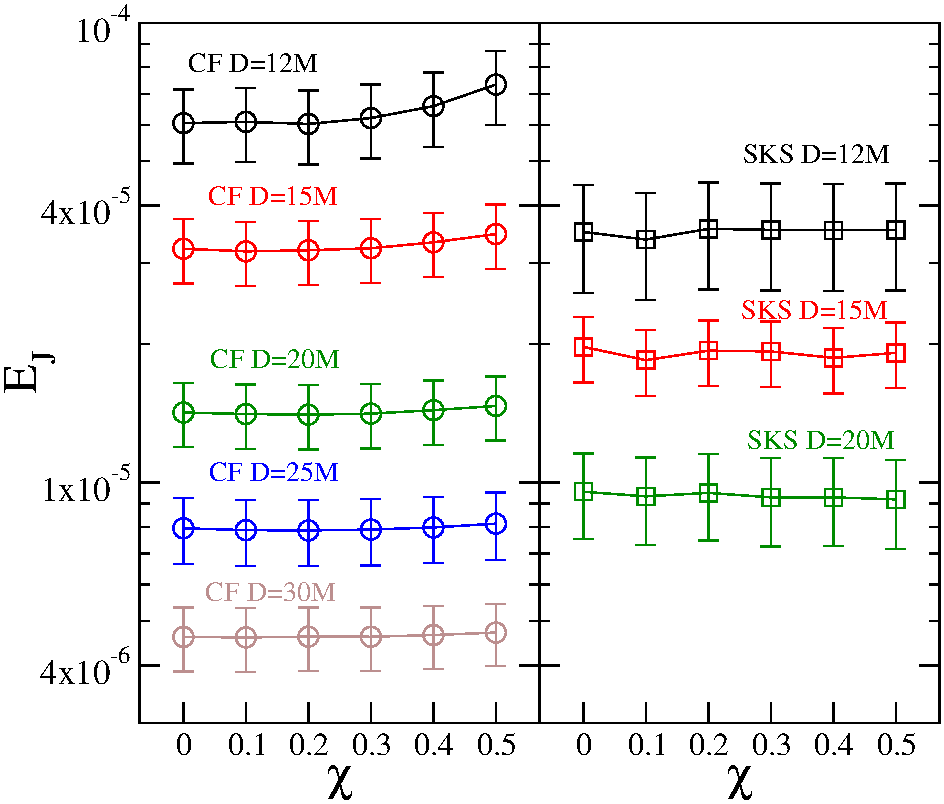
\includegraphics[width=0.95\columnwidth]{chap5/EvsS}
  \caption{Energy in junk radiation as a function of $\chi$ at various
  initial separations, for conformally flat initial data (left panel)
  and SKS initial data (right panel). Within the uncertainty limit,
  there is virtually no dependence of $E_J$ on $\chi$ }
  \label{fig:EvsS}
\end{figure}

Because, as we've shown in Fig.~\ref{fig:EvsS}, there is virtually
no dependence of $E_J$ on $\chi$, in looking at the dependence of
$E_J$ on $D$, we can use a fixed $\chi$; we use
$\chi=0$. Figure~\ref{fig:EvsD} shows $E_J$ as a function of $D$ for
CF and SKS data. Both cases are good fits to power laws. For
conformally flat data,
\begin{equation}
E_J^{\rm CF}\sim 0.06225\left(\frac{D}{M}\right)^{-2.7933}.
\end{equation}
and for SKS data
\begin{equation}
E_J^{\rm SKS}\sim 0.019576\left(\frac{D}{M}\right)^{-2.5464},
\end{equation}
however the latter is just a fit to three data points.

%Figure~\ref{fig:EvsS} shows the energy in junk radiation, $E_J$ as a
%function of a spin. The black curves correspond to conformally flat
%initial data at initial separations of $D=\{12M,15M,20M,25M,30M\}$ and
%the red curves correspond to SKS initial data at initial separations
%of $D=\{12M,15M,20M\}$. Note that this corresponds to all of our data
%from our main runs. It is clear that within the errors of our
%simulations, the junk radiation energy content has virtually no
%dependence on the spin of the black holes. The only exception is that
%for the conformally flat data, $E$ tends to increase as
%$\chi\rightarrow 0.5$. This is most visible in the $D=12M$
%case. Perhaps the dependence of $E_J$ on $\chi$ could become important
%for $\chi>0.5$ if this trend continues.



%Because, as shown in figure~\ref{fig:EvsS}, there is virtually no
%dependence of $E_J$ on $\chi$, in looking at the dependence of $E_J$
%on the initial separation of the black holes, we can look at a fixed
%$\chi$; we choose $\chi=0$. Figure~\ref{fig:EvsD} shows the energy in junk radiation,
%$E_J$ as a function of initial separation, for conformally flat and
%SKS initial data. The dotted lines are the best fit
%power laws to the data. The conformally flat data is a very good fit
%to the power law


\begin{figure}
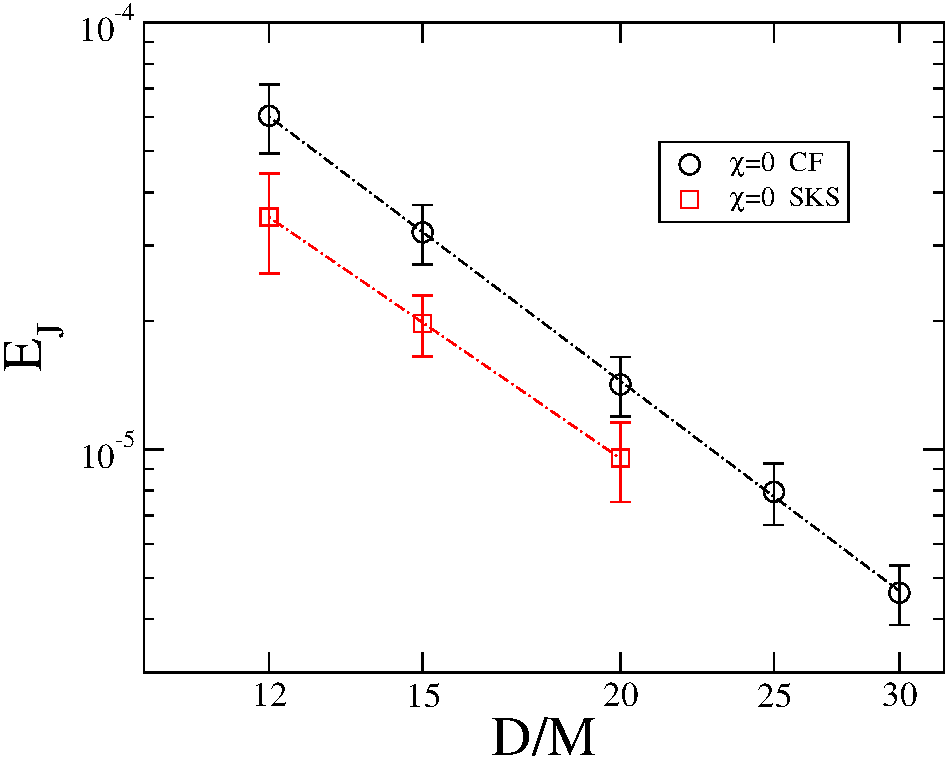
\includegraphics[scale=0.95]{chap5/EvsD}
 \caption{Log-log plot of the energy in junk radiation as a function
   of initial separation for binaries where $\chi=0$. The black circles and red squares denote conformally flat and SKS initial
   data, respectively. The dotted lines are
   power law fits, with indices of $\sim -2.79$ and $\sim
   -2.55$ respectively.}
 \label{fig:EvsD}
\end{figure}

\subsection{Mass Increase}
\label{subsec:MassIncrease}
As discussed earlier, we only attempt to quantify the transient
quantities for CF data, due to the non-convergence of SKS data. We
being by looking at the dependence of $\delta M_{eq}$ on
separation. In Fig.~\ref{fig:MvsD}, we plot it for curves of
constant $\chi$\footnote{we omit $\chi=0$ because the data is too
  noisy}. 

\begin{figure}[!htbp]
\includegraphics[scale=0.95]{chap5/MvsD2}
\caption{$\delta M_{\rm eq}$ as a function of initial separation for
  CF initial data. The dotted lines are the best fits to a power law
  plus a constant offset.}
\label{fig:MvsD}
\end{figure}

The data are nearly independent of distance at high spin, while there
is a clear dependence at lower spin. In each case, we fit the data to
a power law plus a constant offset. The fits are
\begin{eqnarray*}
\delta M_{\rm eq}^{\chi = 0.1} &=&
0.000170\left(D/M\right)^{-1.76}+8.194\times 10^{-7} \\
\delta M_{\rm eq}^{\chi = 0.2} &=&
0.000209\left(D/M\right)^{-1.36}+1.007\times 10^{-5} \\
\delta M_{\rm eq}^{\chi = 0.3} &=&
0.000146\left(D/M\right)^{-0.75}+4.60\times 10^{-5} \\
\delta M_{\rm eq}^{\chi = 0.4} &=&
0.000262\left(D/M\right)^{-0.87}+1.83\times 10^{-4} \\
\delta M_{\rm eq}^{\chi = 0.5} &=&
0.000470\left(D/M\right)^{-0.99}+5.08\times 10^{-4} 
\end{eqnarray*}

In Fig.~\ref{fig:MvsS}, the dependence of $\delta M_{\rm eq}$ is
shown. In general we find that $\delta M_{\rm eq}$ grows rapidly with
$\chi$ and the dependence is nearly exponential at each separation.

\begin{figure}[!htbp]
\includegraphics[scale=0.95]{chap5/MvsS2}
 \caption{$\delta M_{eq}$ as a function of black hole spin $\chi$ for CF
    initial data, evaluated at each different initial separation.}
  \label{fig:MvsS}
\end{figure}



%Finally\note{fix wording}, we can look at the dependence of $\Delta_{S}$ on the initial
%separation of the black holes. To maximize the effect, this is
%evaluated at a constant $\chi=0.5$. This is shown in figure~\ref{fig:MvsD}.
%The data are a good fit to a power law with index $~-5.57$ plus a
%constant offset. However, the constant offset dominates and the data
%vary very little in the parameter space considered.

%\begin{figure}[!htbp]
% \includegraphics[scale=0.50]{MvsD2}
 % \caption{$\Delta M_{eq}$ as a function of initial separation $D$ for CF
  %  initial data, evaluated at $\chi=0.5$ The dotted curve is the best
 % fit power law + constant curve.}
 % \label{fig:MvsD}
%\end{figure}

%Since we have not attempted to model the parameter-space dependence of
%$\Delta M_{eq}$ for SKS initial data, we show only the results for CF
%initial data. In figure~\ref{fig:MvsS} the dependence on $\chi$ is
%shown, at a constant $D=15M$. $\Delta M_{eq}$ grows rapidly with $\chi$ and
%the dependence is nearly exponential.

%\begin{figure}[!htbp]
% \includegraphics[scale=0.50]{MvsS2}
 % \caption{$\Delta M_{eq}$ as a function of black hole spin $\chi$ for CF
  %  initial data, evaluated at $D=15M$. The dotted curve is the best
   % fit exponential curve.}
 % \label{fig:MvsS}
%\end{figure}



\subsection{Spin Decrease}
\label{subsec:SpinDecrease}
As with the mass increase, we only attempt to calculate $\delta S_{\rm
  eq}$ for CF data, as it was found to not be convergent for SKS
data. In Fig.~\ref{fig:SvsD} we plot $\delta S_{\rm eq}$ vs. $D$ for
curves of constant $\chi$\footnote{we omit $\chi=0$ because $\delta
  S_{\rm eq}$ is not well-defined, and we omit $\chi=0.1$ because the
  data is too noisy}. The data are similar to those in
Fig.~\ref{fig:MvsD}, although there is a stronger dependence on separation.

\begin{figure}[!htbp]
 \includegraphics[scale=0.95]{chap5/SvsD2}
  \caption{$\delta S_{\rm eq}$ vs. $D$ for CF initial data. The dotted
    curves are the best fit power law plus constant offsets.}
  \label{fig:SvsD}
\end{figure}

In each case, we fit the data to
a power law plus a constant offset. The fits are
\begin{eqnarray*}
\delta S_{\rm eq}^{\chi = 0.2} &=&
0.000154\left(D/M\right)^{-.966}+5.836\times 10^{-8} \\
\delta S_{\rm eq}^{\chi = 0.3} &=&
0.000340\left(D/M\right)^{-0.836}+6.025\times 10^{-6} \\
\delta S_{\rm eq}^{\chi = 0.4} &=&
0.00136\left(D/M\right)^{-1.189}+8.348\times 10^{-5} \\
\delta S_{\rm eq}^{\chi = 0.5} &=&
0.00261\left(D/M\right)^{-1.133}+3.445\times 10^{-4}
\end{eqnarray*}

In figure~\ref{fig:SvsS}, $\delta S_{\rm eq}$ is plotted as a function
of $\chi$, at different separations. In each case, the data is a good
fit to an exponential; at $D=15M$,
\begin{equation}
\delta S_{\rm eq} \sim 1.563\times10^{-6}e^{11.546\chi}
\end{equation}

\begin{figure}[!htbp]
\includegraphics[scale=0.95]{chap5/SvsS2}
\caption{Semi-log plot of $\delta S_{\rm eq}$ as a function of $\chi$ for CF data. The
  dotted lines are the best fit exponentials.}
\label{fig:SvsS}
\end{figure}


%The dependence of $\Delta S_{eq}$ on the initial separation of the black
%holes is shown in figure ~\ref{fig:SvsD}. We do this for runs where $\chi=0.5$.
%For the CF initial data, we find a good fit a power law with a
%constant offset
%\begin{equation}
%\Delta_S=0.0004139+150.56\left(\frac{D}{M}\right)^{-5.5654}
%\end{equation}
%and we note that for $D>20M$, there is very little dependence on
%$D$. We do not attempt to fit the SKS data, but we note that there is
%a levelling off trend similar to the CF initial data.

%\begin{figure}[!htbp]
% \includegraphics[scale=0.50]{SvsD2}
 % \caption{The dependence of $\Delta S_{eq}$ on the initial separation of
  %  the binaries. The dotted line is the best fit power law plus
   % constant offset to the data, with a power law index of
   % $~-5.57$.\note{Add proper error bars on this fig!}}
  %\label{fig:SvsD}
%\end{figure}

%We begin\note{change wording} by looking at the dependence of $\Delta S_{eq}$ on the spins of
%the black holes. This is shown in figure~\ref{fig:SvsS} for runs where
%$D=15M$, with the black curve as conformally flata initial data, and
%the red curve as SKS initial data. 

%\begin{figure}[!htbp]
%\includegraphics[scale=0.5]{SvsS2}
%\caption{Semi-log plot of the dependence of $\Delta S_{eq}$ on $\chi$. The
%dotted line is the best fit exponential fit to the data}
%\label{fig:SvsS}
%\end{figure}

%In the case of the conformally flat initial data, we find an exponential dependence on
%the spins of the black holes,
%\begin{equation}
%\Delta_S=1.301\times10^{-6}e^{11.672\chi}
%\end{equation}

%\note{change text}For the SKS initial data, we have done runs at an additional three
%points, going up to $\chi=0.8$. Unlike the CF initial data, which has
%a clear exponential dependence on $\chi$, the $\Delta S$ does not seem
%to have any strong dependence on $\chi$, and the oscillations are
%probably due to numerical noise. \note{Need better discussion here}


\section{Summary }

My Summary.
